% Options for packages loaded elsewhere
\PassOptionsToPackage{unicode}{hyperref}
\PassOptionsToPackage{hyphens}{url}
\PassOptionsToPackage{dvipsnames,svgnames*,x11names*}{xcolor}
%
\documentclass[
  10pt,
  ignorenonframetext,
  x11names, dvipsnames, bibspacing,natbib, table]{beamer}
\usepackage{pgfpages}
\setbeamertemplate{caption}[numbered]
\setbeamertemplate{caption label separator}{: }
\setbeamercolor{caption name}{fg=normal text.fg}
\beamertemplatenavigationsymbolsempty
% Prevent slide breaks in the middle of a paragraph
\widowpenalties 1 10000
\raggedbottom
\setbeamertemplate{part page}{
  \centering
  \begin{beamercolorbox}[sep=16pt,center]{part title}
    \usebeamerfont{part title}\insertpart\par
  \end{beamercolorbox}
}
\setbeamertemplate{section page}{
  \centering
  \begin{beamercolorbox}[sep=12pt,center]{part title}
    \usebeamerfont{section title}\insertsection\par
  \end{beamercolorbox}
}
\setbeamertemplate{subsection page}{
  \centering
  \begin{beamercolorbox}[sep=8pt,center]{part title}
    \usebeamerfont{subsection title}\insertsubsection\par
  \end{beamercolorbox}
}
\AtBeginPart{
  \frame{\partpage}
}
\AtBeginSection{
  \ifbibliography
  \else
    \frame{\sectionpage}
  \fi
}
\AtBeginSubsection{
  \frame{\subsectionpage}
}
\usepackage{amsmath,amssymb}
\usepackage{lmodern}
\usepackage{ifxetex,ifluatex}
\ifnum 0\ifxetex 1\fi\ifluatex 1\fi=0 % if pdftex
  \usepackage[T1]{fontenc}
  \usepackage[utf8]{inputenc}
  \usepackage{textcomp} % provide euro and other symbols
\else % if luatex or xetex
  \usepackage{unicode-math}
  \defaultfontfeatures{Scale=MatchLowercase}
  \defaultfontfeatures[\rmfamily]{Ligatures=TeX,Scale=1}
\fi
\usetheme[]{Rafal_beamerSly1}
% Use upquote if available, for straight quotes in verbatim environments
\IfFileExists{upquote.sty}{\usepackage{upquote}}{}
\IfFileExists{microtype.sty}{% use microtype if available
  \usepackage[]{microtype}
  \UseMicrotypeSet[protrusion]{basicmath} % disable protrusion for tt fonts
}{}
\makeatletter
\@ifundefined{KOMAClassName}{% if non-KOMA class
  \IfFileExists{parskip.sty}{%
    \usepackage{parskip}
  }{% else
    \setlength{\parindent}{0pt}
    \setlength{\parskip}{6pt plus 2pt minus 1pt}}
}{% if KOMA class
  \KOMAoptions{parskip=half}}
\makeatother
\usepackage{xcolor}
\IfFileExists{xurl.sty}{\usepackage{xurl}}{} % add URL line breaks if available
\IfFileExists{bookmark.sty}{\usepackage{bookmark}}{\usepackage{hyperref}}
\hypersetup{
  pdftitle={Taking uncertainty seriously A Bayesian approach to word embedding bias estimation},
  pdfauthor={Alicja Dobrzeniecka \& Rafal Urbaniak (LoPSE research group, University of Gdansk, Vrij Universiteit Amsterdam)},
  colorlinks=true,
  linkcolor=Maroon,
  filecolor=Maroon,
  citecolor=Blue,
  urlcolor=blue,
  pdfcreator={LaTeX via pandoc}}
\urlstyle{same} % disable monospaced font for URLs
\newif\ifbibliography
\usepackage{color}
\usepackage{fancyvrb}
\newcommand{\VerbBar}{|}
\newcommand{\VERB}{\Verb[commandchars=\\\{\}]}
\DefineVerbatimEnvironment{Highlighting}{Verbatim}{commandchars=\\\{\}}
% Add ',fontsize=\small' for more characters per line
\usepackage{framed}
\definecolor{shadecolor}{RGB}{248,248,248}
\newenvironment{Shaded}{\begin{snugshade}}{\end{snugshade}}
\newcommand{\AlertTok}[1]{\textcolor[rgb]{0.94,0.16,0.16}{#1}}
\newcommand{\AnnotationTok}[1]{\textcolor[rgb]{0.56,0.35,0.01}{\textbf{\textit{#1}}}}
\newcommand{\AttributeTok}[1]{\textcolor[rgb]{0.77,0.63,0.00}{#1}}
\newcommand{\BaseNTok}[1]{\textcolor[rgb]{0.00,0.00,0.81}{#1}}
\newcommand{\BuiltInTok}[1]{#1}
\newcommand{\CharTok}[1]{\textcolor[rgb]{0.31,0.60,0.02}{#1}}
\newcommand{\CommentTok}[1]{\textcolor[rgb]{0.56,0.35,0.01}{\textit{#1}}}
\newcommand{\CommentVarTok}[1]{\textcolor[rgb]{0.56,0.35,0.01}{\textbf{\textit{#1}}}}
\newcommand{\ConstantTok}[1]{\textcolor[rgb]{0.00,0.00,0.00}{#1}}
\newcommand{\ControlFlowTok}[1]{\textcolor[rgb]{0.13,0.29,0.53}{\textbf{#1}}}
\newcommand{\DataTypeTok}[1]{\textcolor[rgb]{0.13,0.29,0.53}{#1}}
\newcommand{\DecValTok}[1]{\textcolor[rgb]{0.00,0.00,0.81}{#1}}
\newcommand{\DocumentationTok}[1]{\textcolor[rgb]{0.56,0.35,0.01}{\textbf{\textit{#1}}}}
\newcommand{\ErrorTok}[1]{\textcolor[rgb]{0.64,0.00,0.00}{\textbf{#1}}}
\newcommand{\ExtensionTok}[1]{#1}
\newcommand{\FloatTok}[1]{\textcolor[rgb]{0.00,0.00,0.81}{#1}}
\newcommand{\FunctionTok}[1]{\textcolor[rgb]{0.00,0.00,0.00}{#1}}
\newcommand{\ImportTok}[1]{#1}
\newcommand{\InformationTok}[1]{\textcolor[rgb]{0.56,0.35,0.01}{\textbf{\textit{#1}}}}
\newcommand{\KeywordTok}[1]{\textcolor[rgb]{0.13,0.29,0.53}{\textbf{#1}}}
\newcommand{\NormalTok}[1]{#1}
\newcommand{\OperatorTok}[1]{\textcolor[rgb]{0.81,0.36,0.00}{\textbf{#1}}}
\newcommand{\OtherTok}[1]{\textcolor[rgb]{0.56,0.35,0.01}{#1}}
\newcommand{\PreprocessorTok}[1]{\textcolor[rgb]{0.56,0.35,0.01}{\textit{#1}}}
\newcommand{\RegionMarkerTok}[1]{#1}
\newcommand{\SpecialCharTok}[1]{\textcolor[rgb]{0.00,0.00,0.00}{#1}}
\newcommand{\SpecialStringTok}[1]{\textcolor[rgb]{0.31,0.60,0.02}{#1}}
\newcommand{\StringTok}[1]{\textcolor[rgb]{0.31,0.60,0.02}{#1}}
\newcommand{\VariableTok}[1]{\textcolor[rgb]{0.00,0.00,0.00}{#1}}
\newcommand{\VerbatimStringTok}[1]{\textcolor[rgb]{0.31,0.60,0.02}{#1}}
\newcommand{\WarningTok}[1]{\textcolor[rgb]{0.56,0.35,0.01}{\textbf{\textit{#1}}}}
\usepackage{longtable,booktabs,array}
\usepackage{calc} % for calculating minipage widths
\usepackage{caption}
% Make caption package work with longtable
\makeatletter
\def\fnum@table{\tablename~\thetable}
\makeatother
\setlength{\emergencystretch}{3em} % prevent overfull lines
\providecommand{\tightlist}{%
  \setlength{\itemsep}{0pt}\setlength{\parskip}{0pt}}
\setcounter{secnumdepth}{-\maxdimen} % remove section numbering
\ifluatex
  \usepackage{selnolig}  % disable illegal ligatures
\fi
\newlength{\cslhangindent}
\setlength{\cslhangindent}{1.5em}
\newlength{\csllabelwidth}
\setlength{\csllabelwidth}{3em}
\newenvironment{CSLReferences}[2] % #1 hanging-ident, #2 entry spacing
 {% don't indent paragraphs
  \setlength{\parindent}{0pt}
  % turn on hanging indent if param 1 is 1
  \ifodd #1 \everypar{\setlength{\hangindent}{\cslhangindent}}\ignorespaces\fi
  % set entry spacing
  \ifnum #2 > 0
  \setlength{\parskip}{#2\baselineskip}
  \fi
 }%
 {}
\usepackage{calc}
\newcommand{\CSLBlock}[1]{#1\hfill\break}
\newcommand{\CSLLeftMargin}[1]{\parbox[t]{\csllabelwidth}{#1}}
\newcommand{\CSLRightInline}[1]{\parbox[t]{\linewidth - \csllabelwidth}{#1}\break}
\newcommand{\CSLIndent}[1]{\hspace{\cslhangindent}#1}

\title{\Large Taking uncertainty seriously \newline \normalsize A
Bayesian approach to word embedding bias estimation}
\author{Alicja Dobrzeniecka \& Rafal Urbaniak
\footnotesize \newline (LoPSE research group, University of Gdansk, Vrij
Universiteit Amsterdam)}
\date{Boston, April Fools' Day}

\begin{document}
\frame{\titlepage}

\begin{frame}{Presentation plan}
\protect\hypertarget{presentation-plan}{}
\begin{itemize}
\tightlist
\item
  Bias in word embeddings
\item
  WEAT and MAC methods
\item
  Methodological problems
\item
  Limitations of pre-averaging in bias detection methods
\item
  Accounting for uncertainty with Bayesian approach
\end{itemize}
\end{frame}

\begin{frame}{Word2vec}
\protect\hypertarget{word2vec}{}
\begin{block}{Question}
\protect\hypertarget{question}{}
How to sensibly represent words with numbers?

\pause
\end{block}

\begin{block}{One-hot encoding}
\protect\hypertarget{one-hot-encoding}{}
Well, you could use 30k binary vectors with a slot for each lexical
unit\dots

\pause

\dots \dots but this would be inefficient and wouldn't capture any
relations between words.
\end{block}
\end{frame}

\begin{frame}{Word2vec}
\protect\hypertarget{word2vec-1}{}
\begin{center}
 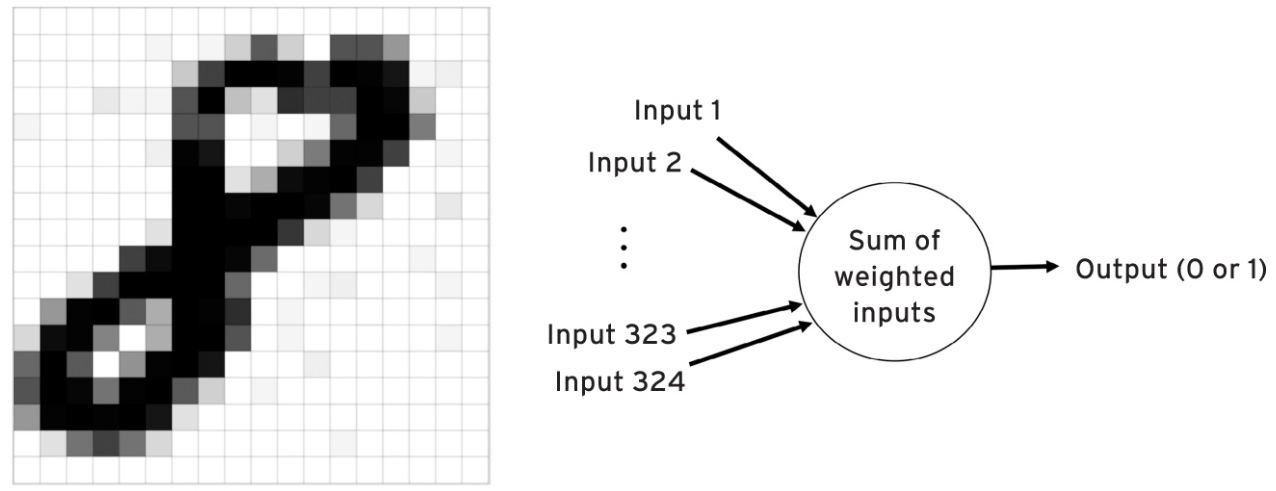
\includegraphics[width = 9cm]{images/perceptron1.png}
\end{center}

\vspace{-3mm}

\tiny \hfill \color{gray}Illustration: M. Mitchell \color{black}

\footnotesize

\begin{block}{Rosenblatt's perceptron}
\begin{itemize}
\item Inputs (pixel intensities) with weights
\item Nodes with activation levels from 0-1
\item (Perhaps) 0-1 output based on a threshold
\end{itemize}
\end{block}
\end{frame}

\begin{frame}{Word2vec}
\protect\hypertarget{word2vec-2}{}
\begin{center}
 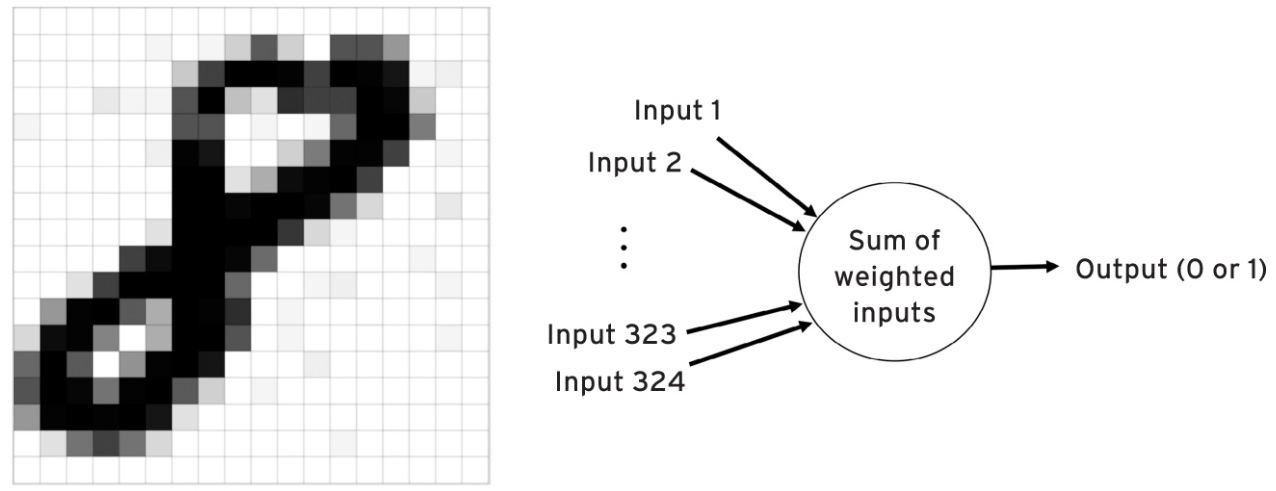
\includegraphics[width = 9cm]{images/perceptron1.png}
\end{center}

\vspace{-3mm}

\tiny \hfill \color{gray}Illustration: M. Mitchell \color{black}

\footnotesize

\begin{block}{Learning}
\begin{itemize}
\item Start with random weights
\item Test on a case:
\begin{itemize}
\item If right, don't change weights.
\item If wrong, change weights a bit, with focus on the ones more responsible for the judgment:
\begin{align*}
w_j & \leftarrow w_j = \overbrace{\eta}^{\text{learning rate}}(\underbrace{t}_{\text{correct output}} - \overbrace{y}^{\text{actual output}})\underbrace{x_j}_{\text{actual input}}
\end{align*}
\end{itemize}
\end{itemize}

\end{block}
\end{frame}

\begin{frame}{Word2vec}
\protect\hypertarget{word2vec-3}{}
\begin{columns}
\column{0.45\linewidth}
    
    

\begin{center}
 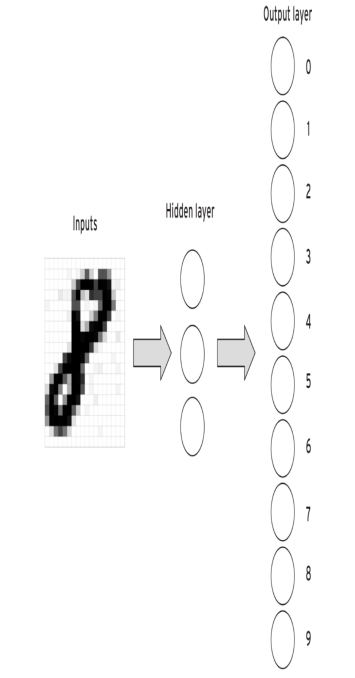
\includegraphics[height = 6cm, width = 5cm]{images/perceptron2.png}
\end{center}


\vspace{-3mm}
\tiny \hfill \color{gray}Illustration: M. Mitchell \color{black}



\column{0.5\linewidth}

\footnotesize 

\begin{itemize}
\item Each hidden unit takes a weighted sum of 324 inputs and passes on its activation level as input to outer layer units. 

\item Activation levels of outer layers are interpreted as network's levels of confidence in a classification problem.

\item Learning: back-propagation (gradient descent: approximate  the direction of steepest descent in the error surface w.r.t to weights, modify accordingly).
\end{itemize}

\end{columns}
\end{frame}

\begin{frame}{Word2vec}
\protect\hypertarget{word2vec-4}{}
\begin{block}{Distributional semantics}
\protect\hypertarget{distributional-semantics}{}
\begin{itemize}
\item "You shall know a word by the company it keeps" (John Firth, 1957)


\item "the degree of semantic similarity between two linguistic expressions $A$ and $B$ is a function of the similarity of the linguistic contexts in which $A$ and $B$ can appear." (A. Lenci, 2008)


\end{itemize}

\pause

\begin{center}
 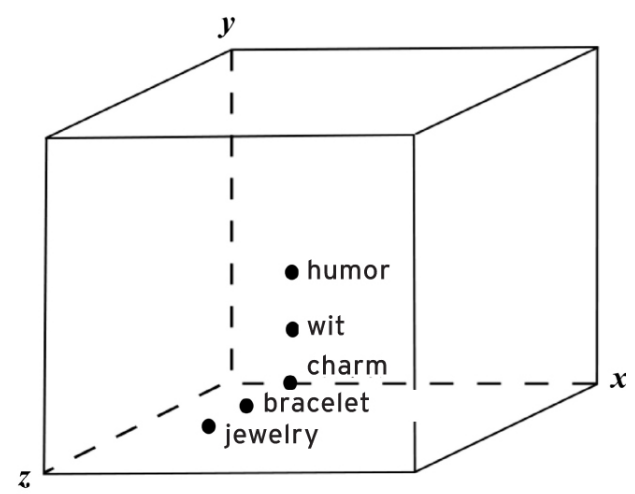
\includegraphics[height = 5cm, width = 5cm]{images/similarity1.png}
\end{center}

\vspace{-3mm}

\tiny \hfill \color{gray}Illustration: M. Mitchell \color{black}
\end{block}
\end{frame}

\begin{frame}{Word2vec}
\protect\hypertarget{word2vec-5}{}
\begin{block}{Google and Mikolov}
\protect\hypertarget{google-and-mikolov}{}
\emph{Efficient Estimation of Word Representation in Vector Space}, 2013

Let's train a neural network and use vectors of weights!

\begin{center}
 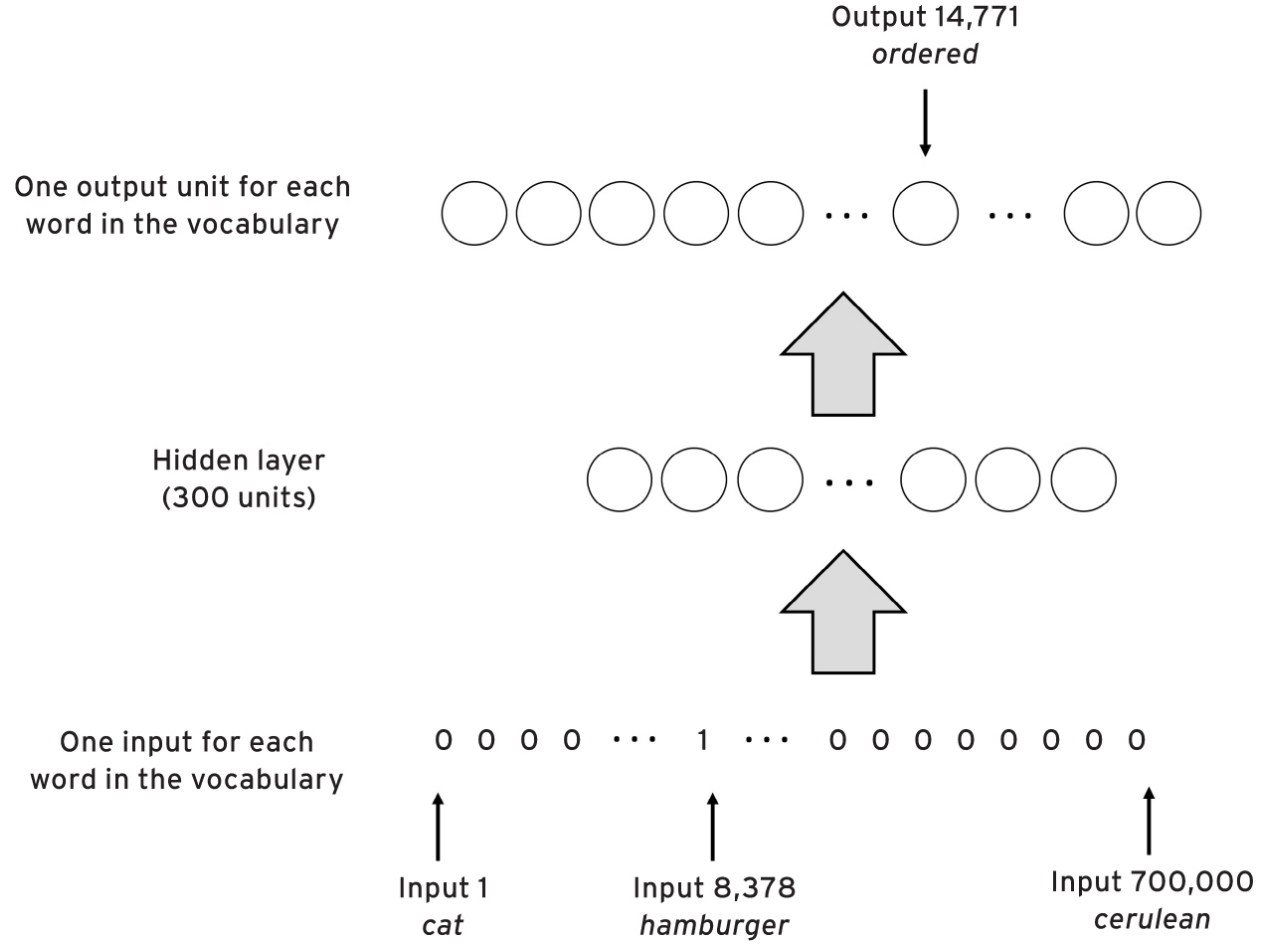
\includegraphics[height = 5cm, width = 6cm]{images/word2vec1.png}
\end{center}

\vspace{-3mm}

\tiny \hfill \color{gray}Illustration: M. Mitchell \color{black}
\end{block}
\end{frame}

\begin{frame}{Word2vec}
\protect\hypertarget{word2vec-6}{}
\begin{block}{Google and Mikolov}
\protect\hypertarget{google-and-mikolov-1}{}
\emph{Efficient Estimation of Word Representation in Vector Space}, 2013

Let's train a neural network and use vectors of weights!

\begin{center}
 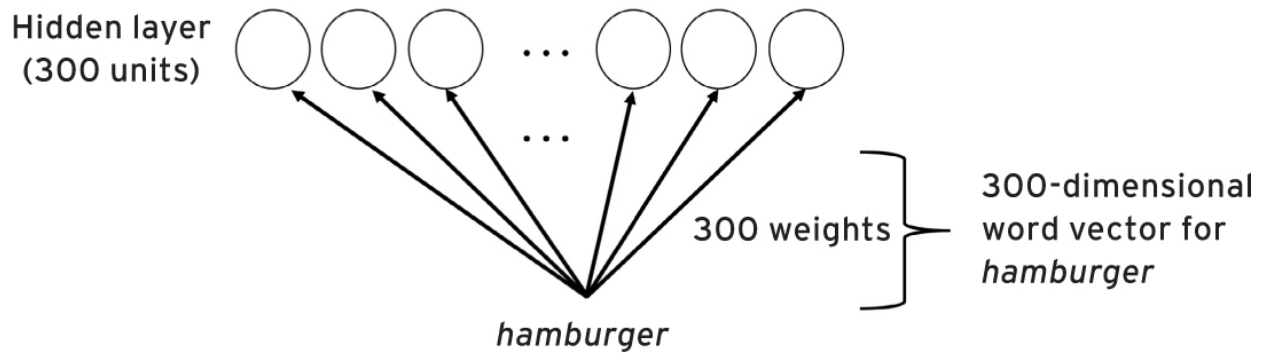
\includegraphics[height = 3cm, width = 7cm]{images/word2vec2.png}
\end{center}

\vspace{-3mm}

\tiny \hfill \color{gray}Illustration: M. Mitchell \color{black}
\end{block}
\end{frame}

\begin{frame}{Word2vec}
\protect\hypertarget{word2vec-7}{}
\begin{longtable}[]{@{}llllll@{}}
\toprule
word & 1 & 2 & 3 & 4 & \ldots{} \\
\midrule
\endhead
woman & 0.456 & 0.267 & 0.675 & 0.131 & \ldots{} \\
man & 0.451 & 0.897 & 0.472 & 0.088 & \ldots{} \\
\bottomrule
\end{longtable}

\begin{block}{Question}
\protect\hypertarget{question-1}{}
How is this supposed to capture semantic relations?

\pause
\end{block}

\begin{block}{General idea}
\protect\hypertarget{general-idea}{}
Similarity in vector direction.
\end{block}
\end{frame}

\begin{frame}{Cosine similarity}
\protect\hypertarget{cosine-similarity}{}
\begin{columns}
\column{0.45\linewidth}
    

\begin{center}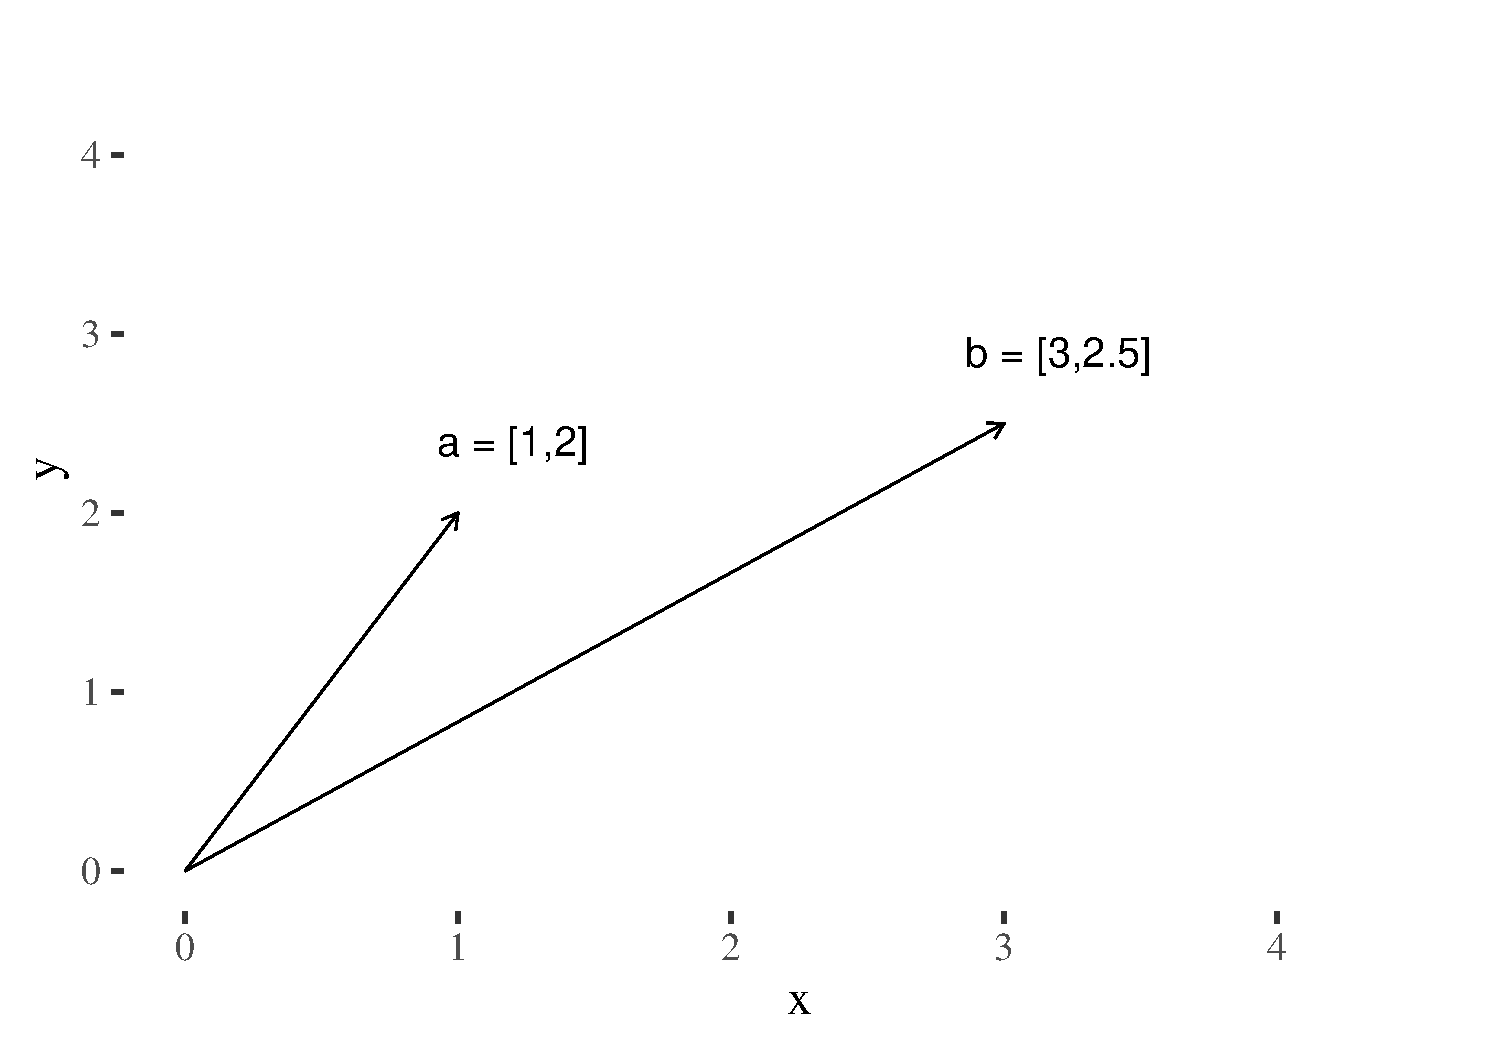
\includegraphics[width=1\linewidth]{presentationBoston_files/figure-beamer/cosine1-1} \end{center}


\column{0.5\linewidth}

\footnotesize 

\begin{block}{Vectors}
\begin{align*}
a  & = [1,2]\\
b  &= [3,2.5]
\end{align*}

\end{block}
\pause 

\begin{block}{Dot product}


\begin{align*}
a \cdot b & = a_1 b_1 + a_2 b_2\\
a \cdot a & = a_1^2 + a_2 ^ 2 \\
\lVert a\rVert & = \sqrt{(a \cdot a)}
\end{align*}

\end{block}



\end{columns}
\end{frame}

\begin{frame}{Cosine similarity}
\protect\hypertarget{cosine-similarity-1}{}
\begin{columns}
\column{0.45\linewidth}
    

\begin{center}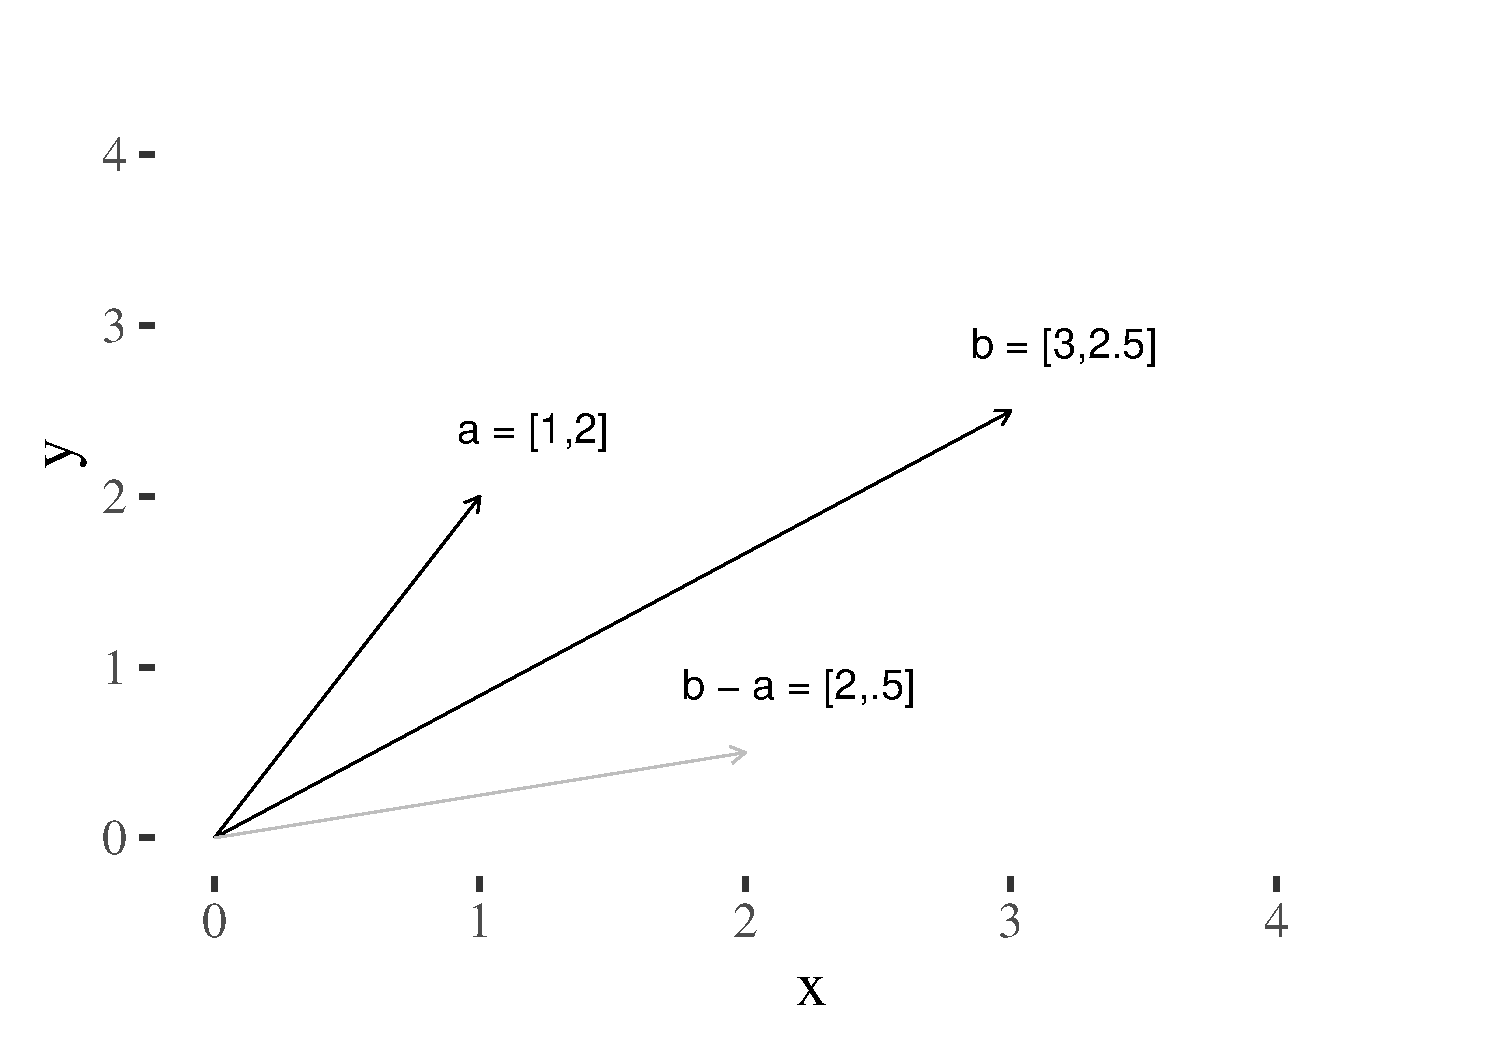
\includegraphics[width=1\linewidth]{presentationBoston_files/figure-beamer/cosine2-1} \end{center}


\column{0.5\linewidth}

\footnotesize 


\begin{block}{Vectors}

\begin{align*}
a  & = [1,2]\\
b  &= [3,2.5]
\end{align*}

\end{block}


\begin{block}{Dot product}

\begin{align*}
a \cdot b & = a_1 b_1 + a_2 b_2\\
a \cdot a & = a_1^2 + a_2 ^ 2 \\
\lVert a\rVert & = \sqrt{(a \cdot a)}
\end{align*}

\end{block}


\begin{block}{Vector difference}

\begin{align*}
b - a & = [b_1- a_1, b_2 - a_2 ]
\end{align*}

\end{block}

\end{columns}
\end{frame}

\begin{frame}{Cosine similarity}
\protect\hypertarget{cosine-similarity-2}{}
\begin{columns}
\column{0.45\linewidth}
    

\begin{center}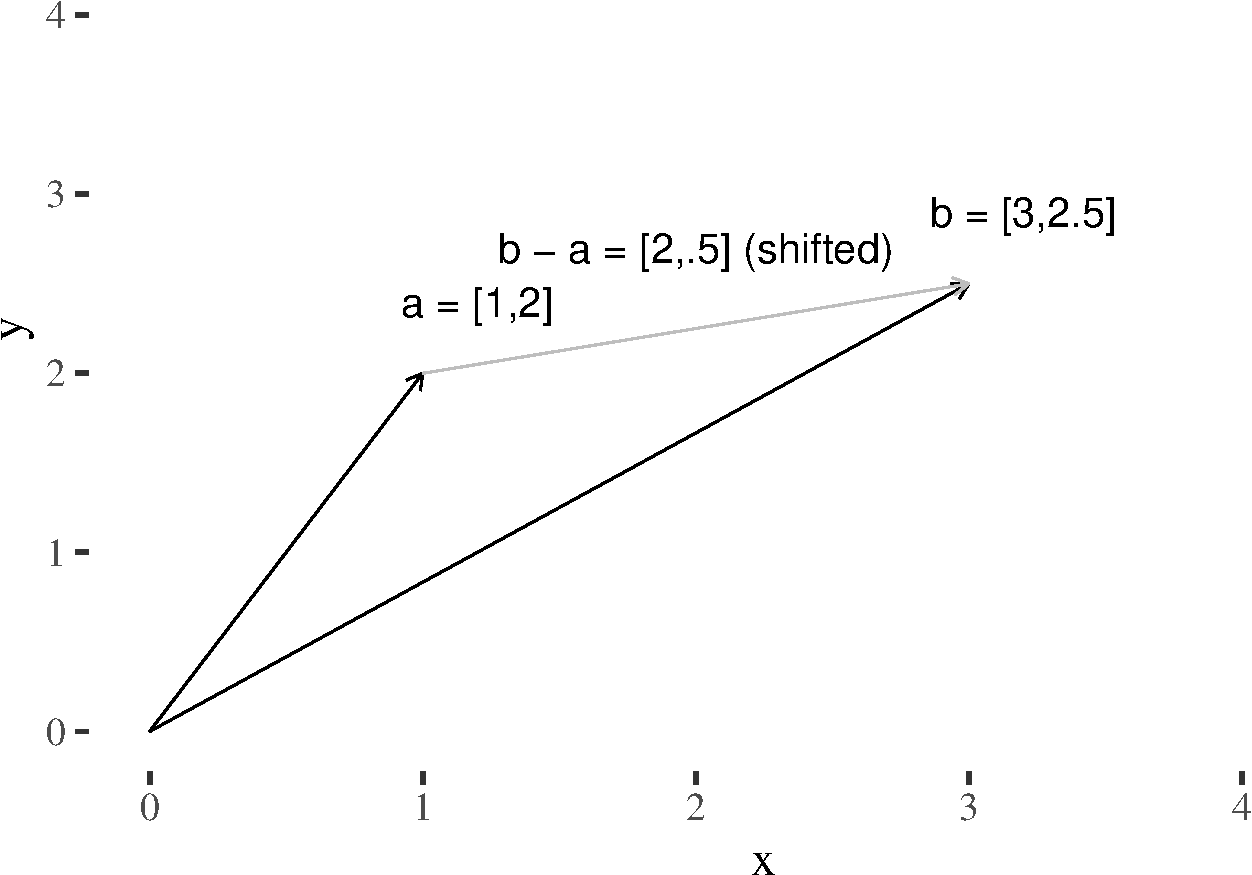
\includegraphics[width=1\linewidth]{presentationBoston_files/figure-beamer/cosine3-1} \end{center}



\column{0.5\linewidth}

\footnotesize 


\begin{block}{Vectors}

\begin{align*}
a  & = [1,2]\\
b  &= [3,2.5]
\end{align*}

\end{block}


\begin{block}{Dot product}

\begin{align*}
a \cdot b & = a_1 b_1 + a_2 b_2\\
a \cdot a & = a_1^2 + a_2 ^ 2 \\
\lVert a\rVert & = \sqrt{(a \cdot a)}
\end{align*}

\end{block}


\begin{block}{Vector difference}

\begin{align*}
b - a & = [b_1- a_1, b_2 - a_2 ]
\end{align*}

\end{block}

\end{columns}
\end{frame}

\begin{frame}{Cosine similarity}
\protect\hypertarget{cosine-similarity-3}{}
\begin{columns}
\column{0.45\linewidth}
    

\begin{center}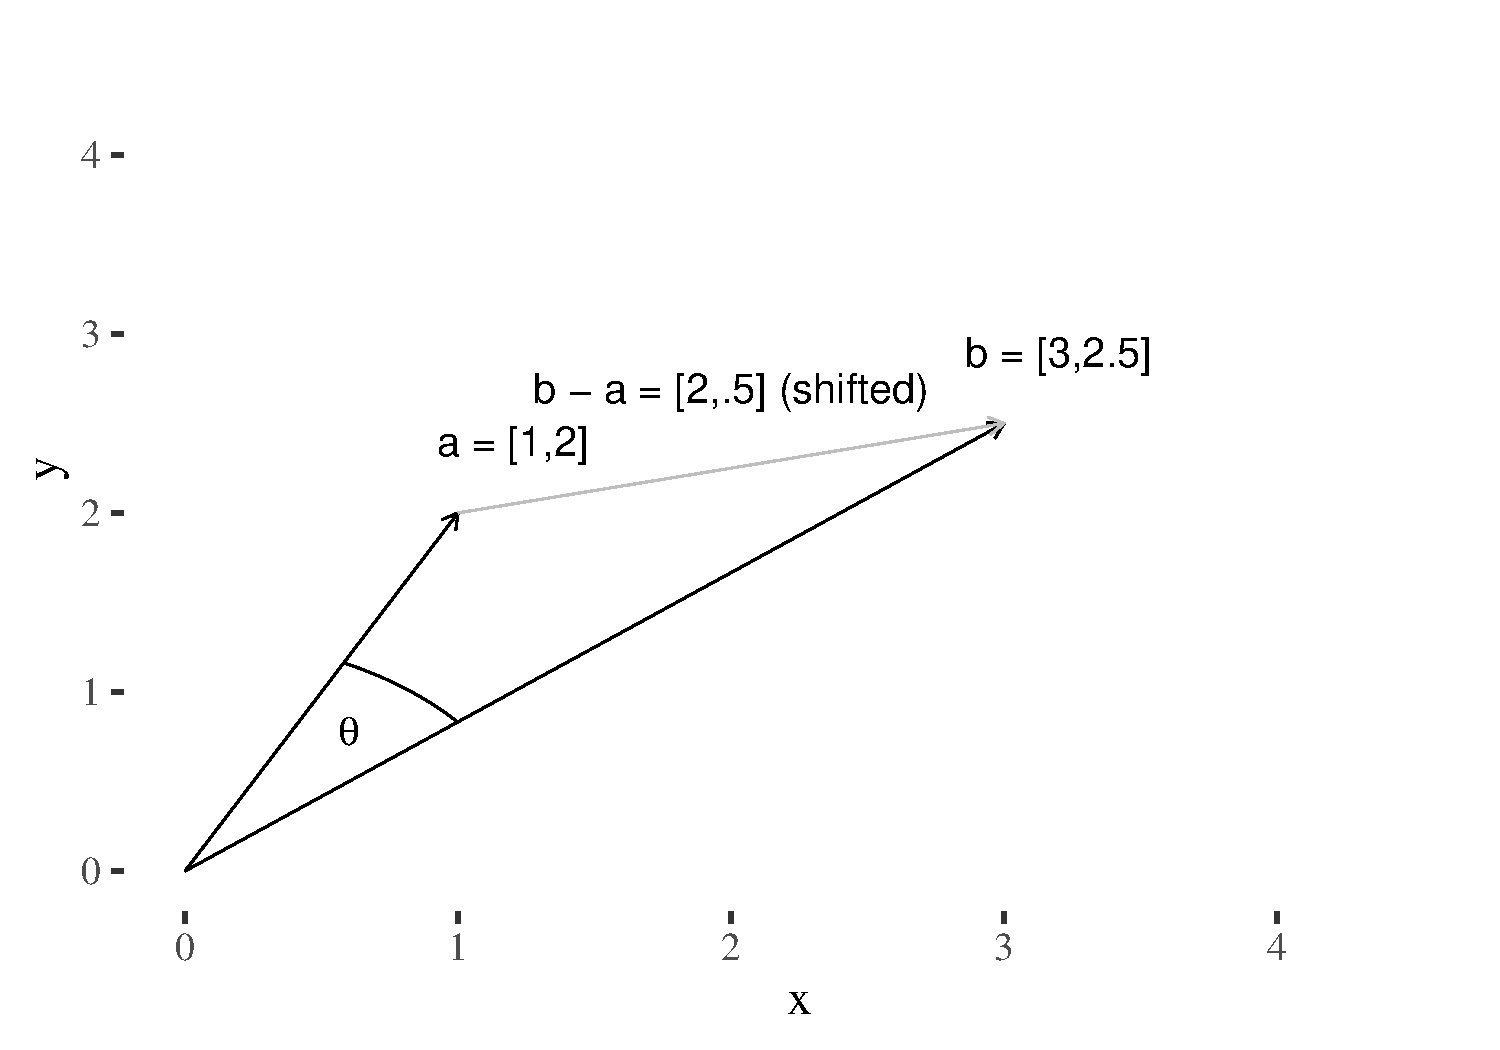
\includegraphics[width=1\linewidth]{presentationBoston_files/figure-beamer/cosine4-1} \end{center}



\column{0.5\linewidth}

\footnotesize 


\begin{block}{Angle}

\begin{align*}
\lVert b - a \rVert^2 &  = \lVert  b \rVert^2 + \lVert a \rVert^2 - 
  2 \lVert b \rVert   \lvert  a \rVert  \cos \theta  \\
b \cdot a  & = \lVert b\rVert \lVert  a \rVert \cos \theta \\ 
\cos \theta & = \frac{b \cdot a}{\lVert b\rVert  \lVert  a \rVert }
\end{align*}

\end{block}


\pause 

\begin{block}{Orthogonality}
\begin{align*}
\cos ( 90^{\circ}) & = 0 \\ 
\frac{b \cdot a}{\lVert  b\rVert \lVert a \rVert} & = 0\\ 
 b \cdot a & = 0  
\end{align*}
\end{block}







\end{columns}
\end{frame}

\begin{frame}{Cosine similarity \& distance}
\protect\hypertarget{cosine-similarity-distance}{}
\vspace{-4mm}

\begin{align} \tag{Sim}
\mathsf{cosineSimilarity}(A,B) & = \frac{A \cdot B}{\lVert  A \rVert \,\lVert B \rVert}
\\
\tag{Distance}
\mathsf{cosineDistance}(A,B) &  = 1 - \mathsf{cosineSimilarity}(A,B)
\end{align}

\begin{itemize}
\item
  Naive interpretation: proximity corresponds to semantic similarity
\item
  Geometric interpretation: direction \(\mathsf{cos} \in (-1,1)\)

  \begin{itemize}
  \tightlist
  \item
    \(1\): maximally smilar
  \item
    \(-1\): opposites
  \item
    \(0\): dissimilar
  \end{itemize}
\item
  \(\mathsf{cosineDistance}\in (0, 2)\)
\end{itemize}
\end{frame}

\begin{frame}{Cosine similarity \& distance}
\protect\hypertarget{cosine-similarity-distance-1}{}
\begin{center}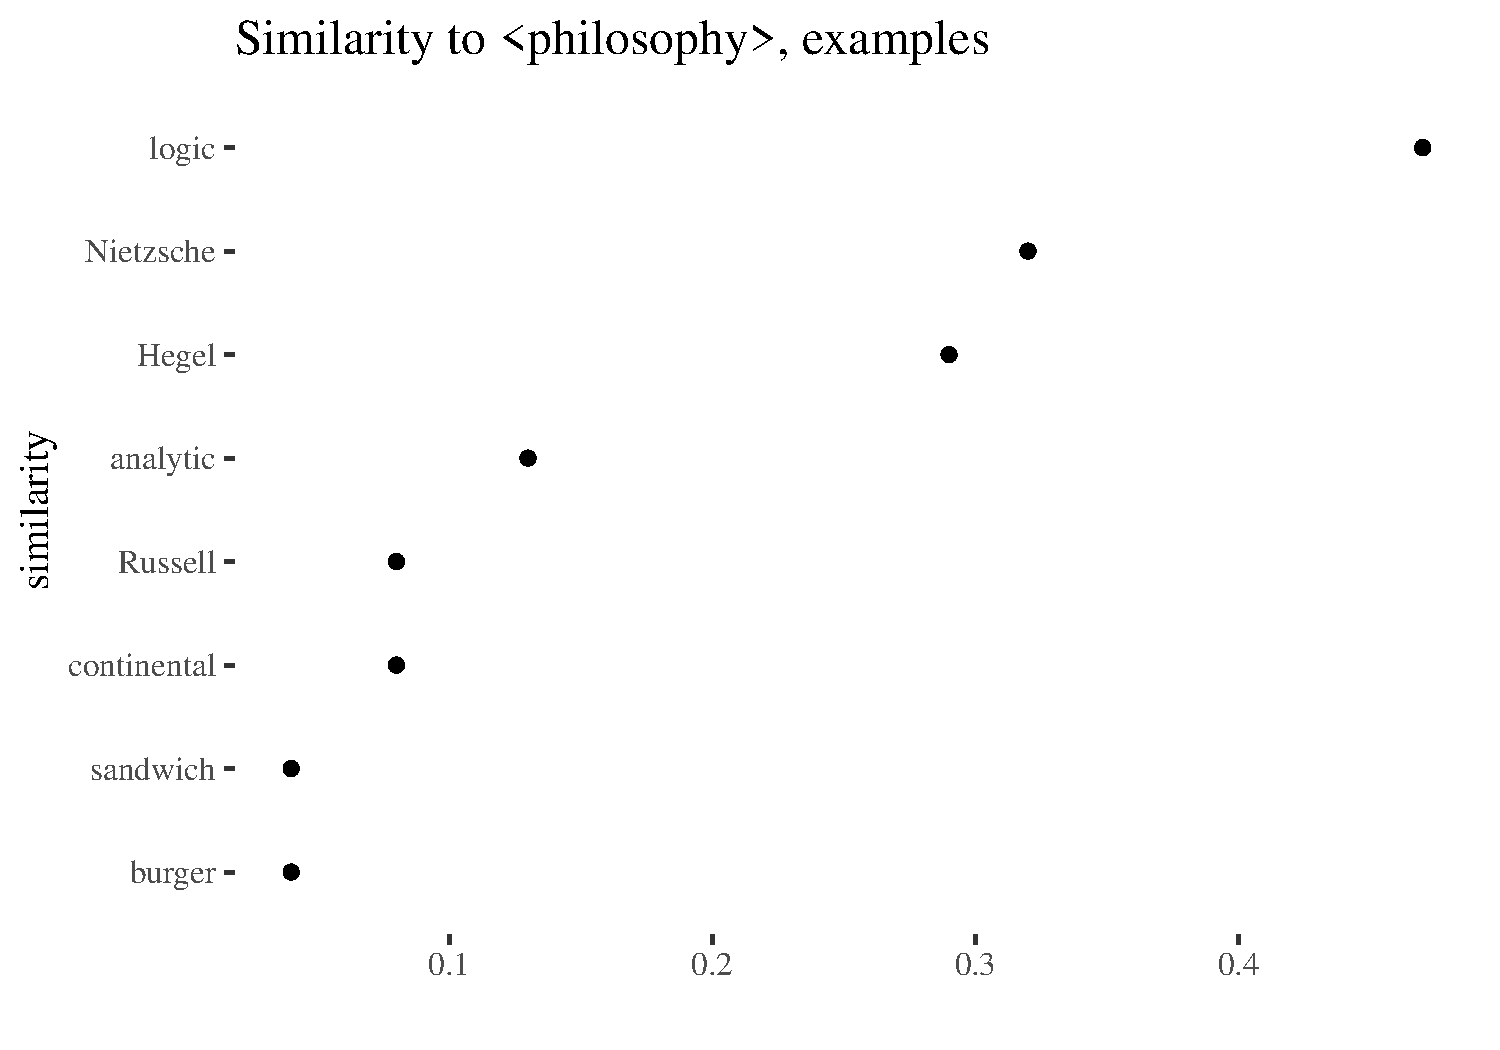
\includegraphics[width=0.8\linewidth]{presentationBoston_files/figure-beamer/philosophy-1} \end{center}

\pause

\begin{block}{The only ``jobs'' in top-tens}
\protect\hypertarget{the-only-jobs-in-top-tens}{}
\begin{itemize}
\item
  Man: robber (.55)
\item
  Woman: policewoman (.6)
\end{itemize}
\end{block}
\end{frame}

\begin{frame}{Cosine-based measures of bias}
\protect\hypertarget{cosine-based-measures-of-bias}{}
\begin{block}{The worry}
\protect\hypertarget{the-worry}{}
Word embeddings can learn implicit harmful biases

\pause
\end{block}

\begin{block}{The basic intuition}
\protect\hypertarget{the-basic-intuition}{}
Stereotypically connected words are cosine-close
\end{block}
\end{frame}

\begin{frame}{Cosine-based measures of bias}
\protect\hypertarget{cosine-based-measures-of-bias-1}{}
\begin{block}{A visual example}
\protect\hypertarget{a-visual-example}{}
\footnotesize

\begin{itemize}
\item
  ``feminine'' occupations: ``homemaker,'' ``nurse,'' ``receptionist,''
  ``librarian,'' etc.
\item
  ``masculine'' occupations: ``maestro,'' ``captain,'' ``architect,''
  ``boss,'' etc.
\end{itemize}

\normalsize

\vspace{1mm}
\footnotesize

\begin{center}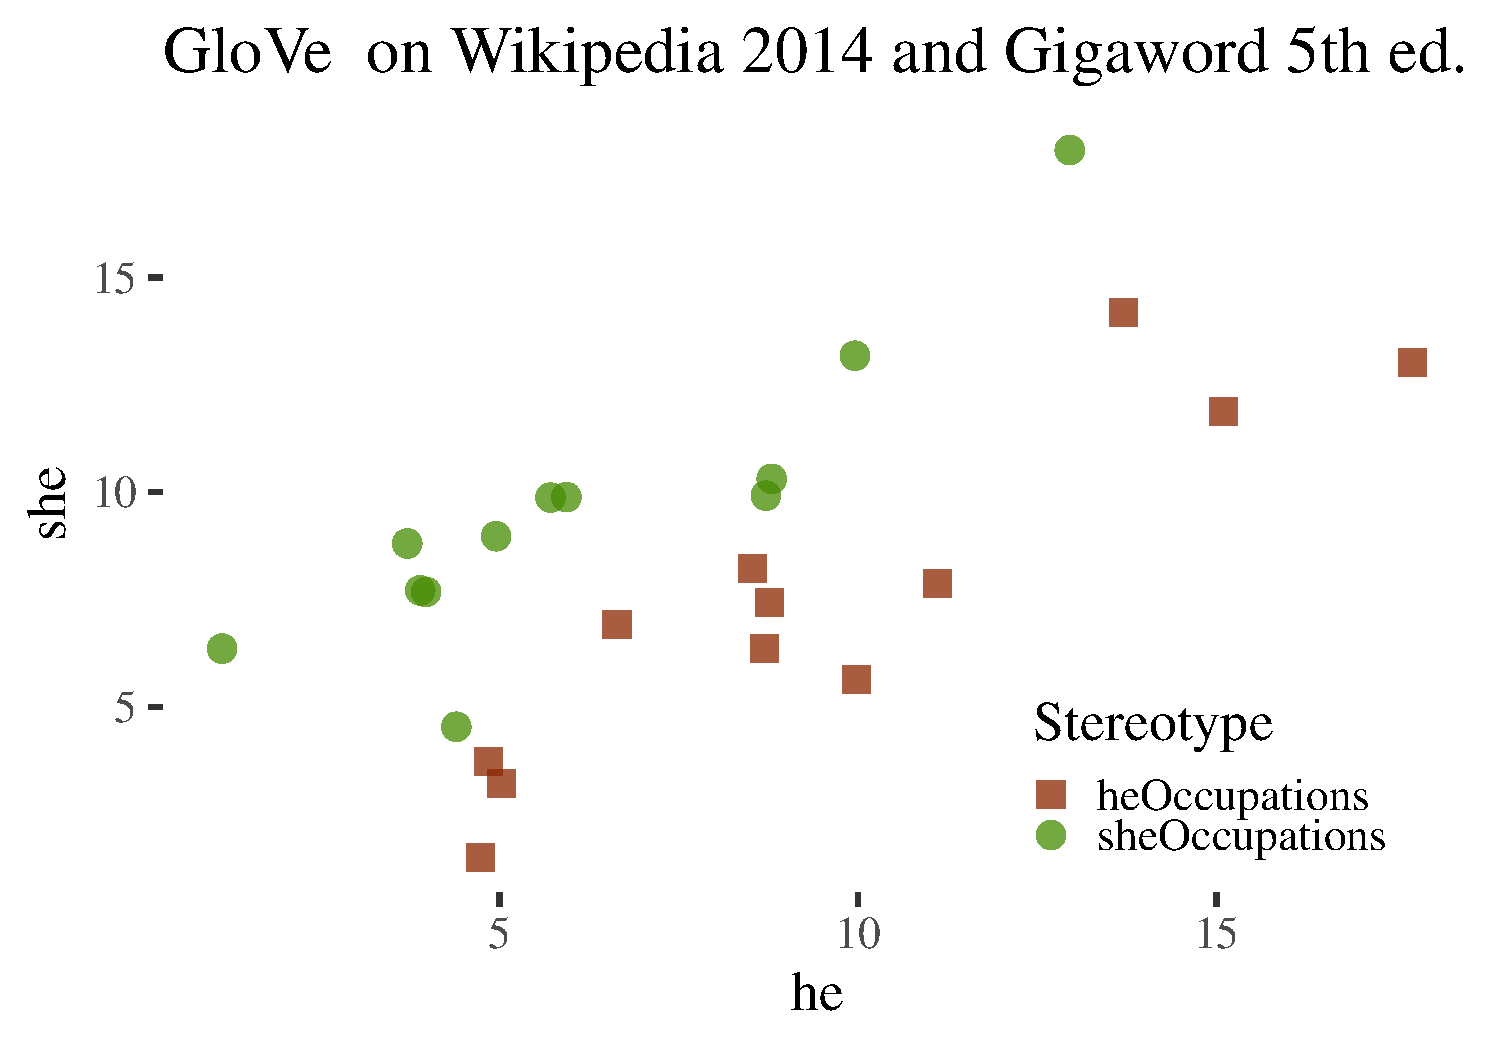
\includegraphics[width=0.6\linewidth]{presentationBoston_files/figure-beamer/unnamed-chunk-1-1} \end{center}
\normalsize
\end{block}
\end{frame}

\begin{frame}{Cosine-based measures of bias}
\protect\hypertarget{cosine-based-measures-of-bias-2}{}
\begin{block}{Example: Word Embedding Association Test (WEAT)}
\protect\hypertarget{example-word-embedding-association-test-weat}{}
\vspace{1mm}
\footnotesize

\begin{center}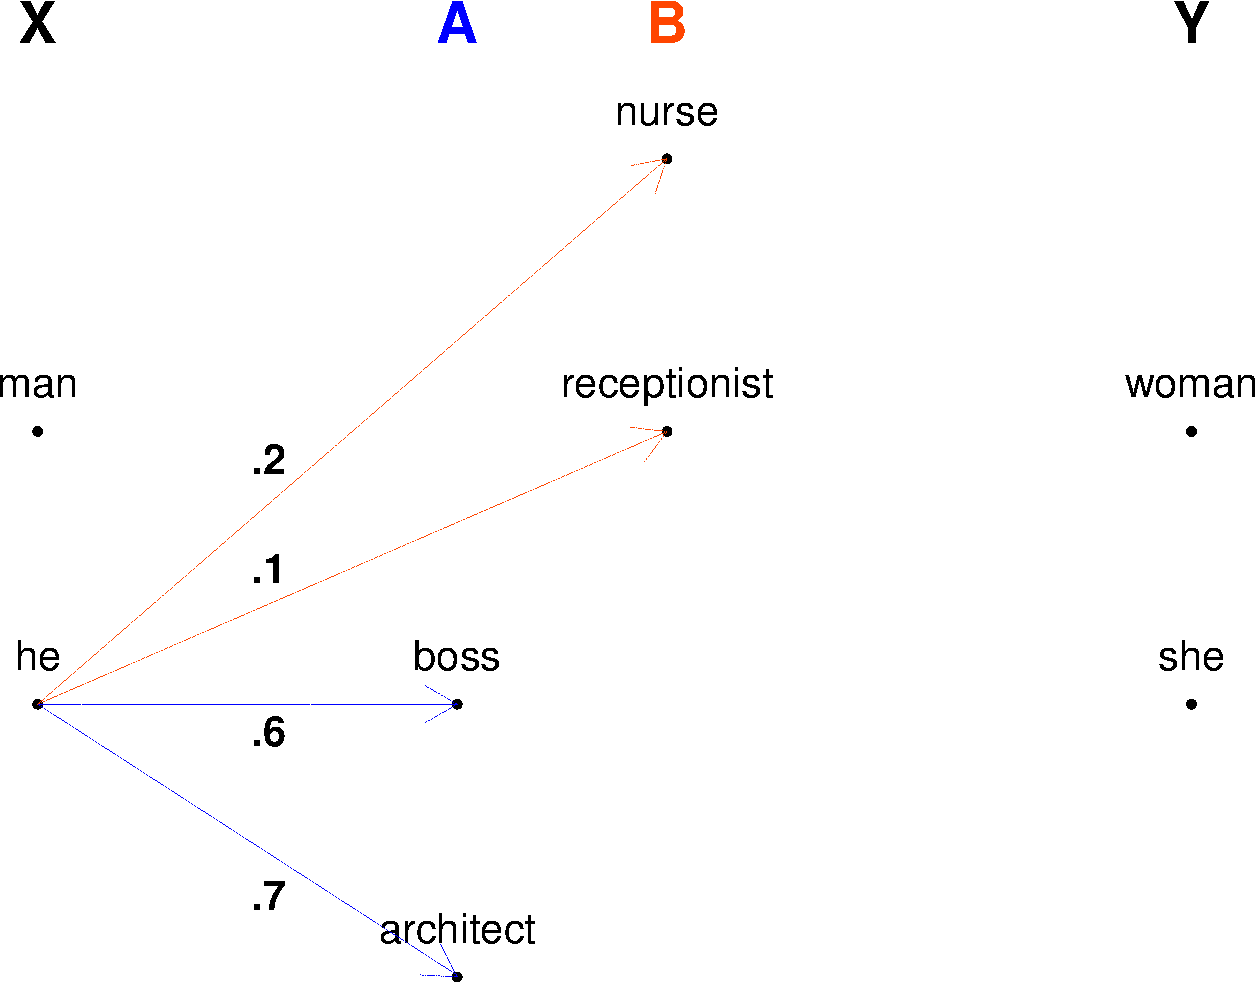
\includegraphics[width=0.55\linewidth]{presentationBoston_files/figure-beamer/unnamed-chunk-2-1} \end{center}
\normalsize

\pause

\footnotesize

\begin{itemize}
\item
  \(s_1 = s(he,A,B) = \frac{.6+.7}{2} - \frac{.2+.1}{2} = .65-.15= .5\)
\item
  \(s_2 = s(man,A,B) = .3\),
  \linebreak  \(s_3 = s(woman,A,B) = -.6, s_4 = s(she, A, B) = -.3\)
\end{itemize}

\vspace{-4mm}

\normalsize

\begin{align*}
\mathsf{WEAT}(A,B) & = \frac{\nicefrac{(s_1+s_2)}{2} - \nicefrac{(s_3+s_4)}{2}}{sd(\{s_1,s_2,s_3,s_4\})} \approx 1.93
\end{align*}
\end{block}
\end{frame}

\begin{frame}{Cosine-based measures of bias}
\protect\hypertarget{cosine-based-measures-of-bias-3}{}
\begin{block}{Example: Word Embedding Association Test (WEAT)}
\protect\hypertarget{example-word-embedding-association-test-weat-1}{}
\begin{align*}
s(t,A,B) & = \frac{\sum_{a\in A}f(t,a)}{\vert A\vert} - \frac{\sum_{b\in B}f(t,b)}{\vert B\vert}
\\
WEAT(A,B) & = \frac{
\mu\left(\{s(x,A,B)\}_{x\in X}\right) -\mu\left(\{s(y,A,B)\}_{y\in Y}\right) 
}{
\sigma\left(\{s(w,A,B)\}_{w\in X\cup Y}\right)
}
\end{align*}

\begin{itemize}
\item
  \(t\) is a term, \(A, B\) are sets of stereotype attribute words,
  \(X\), \(Y\) are protected group words
\item
  For instance, \(X\) might be a set of male names, \(Y\) a set of
  female names, \(A\) might contain stereotypically male-related career
  words, and \(B\) stereotypically female-related family words
\item
  \(s\)-values are used as datapoints in statistical significance tests
\end{itemize}

\footnotesize

\vspace{2mm}

(\protect\hyperlink{ref-Caliskan2017semanticsBiases}{Caliskan, Bryson,
\& Narayanan, 2017}) with extensions in
(\protect\hyperlink{ref-Lauscher2019multidimensional}{Lauscher \&
Glavas, 2019}) and applications in
(\protect\hyperlink{ref-Garg2018years}{Garg, Schiebinger, Jurafsky, \&
Zou, 2018})
\end{block}
\end{frame}

\begin{frame}{Cosine-based measures of bias}
\protect\hypertarget{cosine-based-measures-of-bias-4}{}
\begin{block}{Our main target: Mean Average Cosine Similarity (MAC)}
\protect\hypertarget{our-main-target-mean-average-cosine-similarity-mac}{}
\vspace{1mm}
\footnotesize

\begin{center}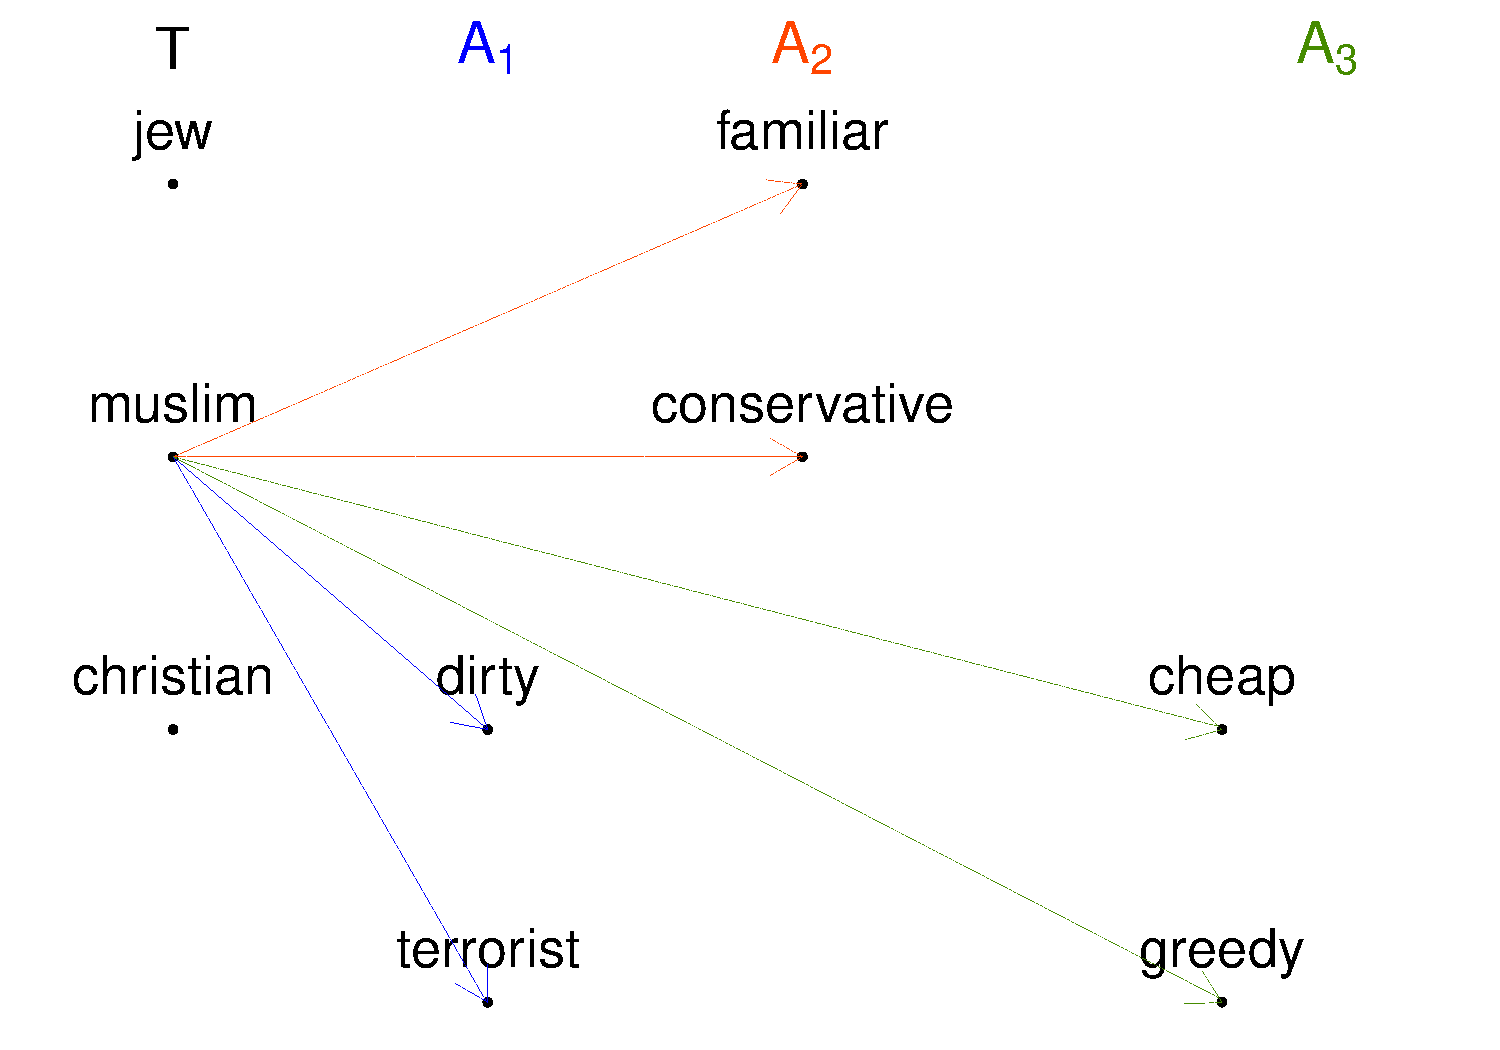
\includegraphics[width=0.5\linewidth]{presentationBoston_files/figure-beamer/unnamed-chunk-3-1} \end{center}
\normalsize

\vspace{-4mm}

\footnotesize

\begin{align*}
 s_1 & = s(muslim,A_1) = \frac{cos(muslim,dirty)+cos(muslim,terrorist)}{2}\\
s_2 & = s(muslim,A_2) = \frac{cos(muslim,familiar)+cos(muslim,conservative)}{2}\\
& \vdots \end{align*}

\vspace{-6mm}

\normalsize

\begin{align*}
 MAC(T,A) & = \mathsf{mean}(\{s_i \vert i \in 1, \dots, k\})
\end{align*}
\end{block}
\end{frame}

\begin{frame}{Cosine-based measures of bias}
\protect\hypertarget{cosine-based-measures-of-bias-5}{}
\begin{block}{Our main target: Mean Average Cosine Similarity (MAC)}
\protect\hypertarget{our-main-target-mean-average-cosine-similarity-mac-1}{}
\begin{align*}
S(t_i, A_j) & = \frac{1}{\vert A_j\vert}\sum_{a\in A_j}\mathsf{cos}(t,a) \\
MAC(T,A) & = \frac{1}{\vert T \vert \,\vert A\vert}\sum_{t_i \in T }\sum_{A_j \in A} S(t_i,A_j)
\end{align*}

\begin{itemize}
\item
  \(T = \{t_1, \dots, t_k\}\) is a class of protected words
\item
  each \(A_j\in A\) is a set of attributes stereotypically associated
  with a protected word
\end{itemize}

\begin{itemize}
\tightlist
\item
  The t-tests they employ are run on average cosines used to calculate
  MAC
\end{itemize}

\vspace{2mm}

\footnotesize

(\protect\hyperlink{ref-Manzini2019blackToCriminal}{Manzini, Lim,
Tsvetkov, \& Black, 2019})
\end{block}
\end{frame}

\begin{frame}{Cosine-based measures of bias}
\protect\hypertarget{cosine-based-measures-of-bias-6}{}
\begin{block}{Our main target: Mean Average Cosine Similarity (MAC)}
\protect\hypertarget{our-main-target-mean-average-cosine-similarity-mac-2}{}
\footnotesize 
\begin{table}

\caption{\label{tab:religionTableHeadEarly}A few rows from the religion dataset}
\centering
\resizebox{\linewidth}{!}{
\begin{tabular}[t]{llrr}
\toprule
protectedWord & wordToCompare & cosineDistance & cosineSimilarity\\
\midrule
jew & greedy & 0.6947042 & 0.3052958\\
rabbi & greedy & 1.0306175 & -0.0306175\\
rabbi & conservative & 0.7175887 & 0.2824113\\
christian & uneducated & 0.5081939 & 0.4918061\\
christianity & cheap & 1.2816164 & -0.2816164\\
muslim & terrorist & 0.2726106 & 0.7273894\\
\bottomrule
\end{tabular}}
\end{table}
\normalsize
\end{block}
\end{frame}

\begin{frame}{Cosine-based measures of bias}
\protect\hypertarget{cosine-based-measures-of-bias-7}{}
\begin{block}{General challenges}
\protect\hypertarget{general-challenges}{}
\begin{itemize}
\tightlist
\item
  Gender-direction: insufficient indicator of bias
  \footnotesize  (\protect\hyperlink{ref-Gonen2019lipstick}{Gonen \&
  Goldberg, 2019})
\end{itemize}

\normalsize

\begin{itemize}
\item
  Use of analogies: unreliable
  \footnotesize  (\protect\hyperlink{ref-Nissim2020fair}{Nissim, Noord,
  \& Goot, 2020}) \normalsize
\item
  High sensitivity to irrelevant factors
  \footnotesize  (\protect\hyperlink{ref-zhang2020robustness}{Zhang,
  Sneyd, \& Stevenson, 2020}) \normalsize
\end{itemize}
\end{block}
\end{frame}

\begin{frame}{Some methodological problems}
\protect\hypertarget{some-methodological-problems}{}
\begin{block}{Word list choice is unprincipled}
\protect\hypertarget{word-list-choice-is-unprincipled}{}
\begin{itemize}
\tightlist
\item
  We run with it for comparison.
\end{itemize}

\pause
\end{block}

\begin{block}{No design considerations to sample size}
\protect\hypertarget{no-design-considerations-to-sample-size}{}
\begin{itemize}
\tightlist
\item
  \protect\hyperlink{ref-Ethayarajh2020measuring}{Ethayarajh}
  (\protect\hyperlink{ref-Ethayarajh2020measuring}{2020}) criticizes
  WEAT uses Bernstein bounds and argues that we would need a bias
  specific dataset of size at least 11903 to claim that the system is
  biased (three times larger than WinoBias).
\end{itemize}

\pause

\begin{itemize}
\tightlist
\item
  We show progress can be made with more sensitive Bayesian methods.
\end{itemize}
\end{block}

\begin{block}{The form of the definition is suspicious}
\protect\hypertarget{the-form-of-the-definition-is-suspicious}{}
\begin{itemize}
\tightlist
\item
  \protect\hyperlink{ref-Ethayarajh2019understanding}{Ethayarajh,
  Duvenaud, \& Hirst}
  (\protect\hyperlink{ref-Ethayarajh2019understanding}{2019}) show that
  if there are two target words only WEAT is always maximal in one
  direction.
\end{itemize}

\pause

\begin{itemize}
\tightlist
\item
  We show the problem runs deeper and stems from pre-averaging, and we
  statistically gauge the uncertainty that arises from raw sample sizes.
\end{itemize}
\end{block}
\end{frame}

\begin{frame}{Some methodological problems}
\protect\hypertarget{some-methodological-problems-1}{}
\begin{block}{No word class distinction and no control group}
\protect\hypertarget{no-word-class-distinction-and-no-control-group}{}
We make the subclasses clear, add human neutral predicates and neutral
predicates for control. We used L2-Reddit corpus and GoogleNews (we
present the results for Reddit for brevity).

\footnotesize 
\begin{table}

\caption{\label{tab:religionTableHeadLate}Rows from extended religion dataset.}
\centering
\resizebox{\linewidth}{!}{
\begin{tabular}[t]{lllrrl}
\toprule
protectedWord & wordToCompare & wordClass & cosineDistance & cosineSimilarity & connection\\
\midrule
torah & hairy & jewish & 1.170 & -0.170 & associated\\
christian & dirty & muslim & 0.949 & 0.051 & different\\
judaism & cheap & jewish & 1.232 & -0.232 & associated\\
christianity & familial & christian & 0.645 & 0.355 & associated\\
mosque & approve & neutral & 0.995 & 0.005 & none\\
imam & carry & human & 0.993 & 0.007 & human\\
mosque & merging & neutral & 0.868 & 0.132 & none\\
muslim & nationalized & neutral & 0.870 & 0.130 & none\\
\bottomrule
\end{tabular}}
\end{table}
\normalsize
\end{block}
\end{frame}

\begin{frame}{Some methodological problems}
\protect\hypertarget{some-methodological-problems-2}{}
\begin{block}{Our neutral words (examples, full list size = ADD)}
\protect\hypertarget{our-neutral-words-examples-full-list-size-add}{}
liquor, pow, ballpark, glitchy, billy, dallas, rip, called, outlooks,
viet, floater, rattlesnake, exports, peruvian, recursion, shortfall,
corrected, amicable, solutions, diagnostic, patently, flops, approx,
percents, lox, catapults, hamburger, engulfed, households, north,
snubbed, playtest
\end{block}

\begin{block}{Our human-related words (examples, full list size = ADD)}
\protect\hypertarget{our-human-related-words-examples-full-list-size-add}{}
switch, studio, stick, soup, sometimes, signal, prior, plant, photo,
path, park, near, menu, latter, grass, clock, wear, walk, visitor, toy,
tissue, throw, talk, speak, sleep, eye, enjoy, blogger, character,
candidate, breakfast, supper, dinner, eat, drink, carry, run, cast, ask,
awake, ear, nose, lunch
\end{block}
\end{frame}

\begin{frame}{Some methodological problems}
\protect\hypertarget{some-methodological-problems-3}{}
\begin{block}{Outliers and surprisingly dissimilar words}
\protect\hypertarget{outliers-and-surprisingly-dissimilar-words}{}
We study those by visualizations and uncertainty estimates.
\end{block}
\end{frame}

\begin{frame}{Some methodological problems}
\protect\hypertarget{some-methodological-problems-4}{}
\begin{block}{Distances for ``muslim''}
\protect\hypertarget{distances-for-muslim}{}
\begin{center}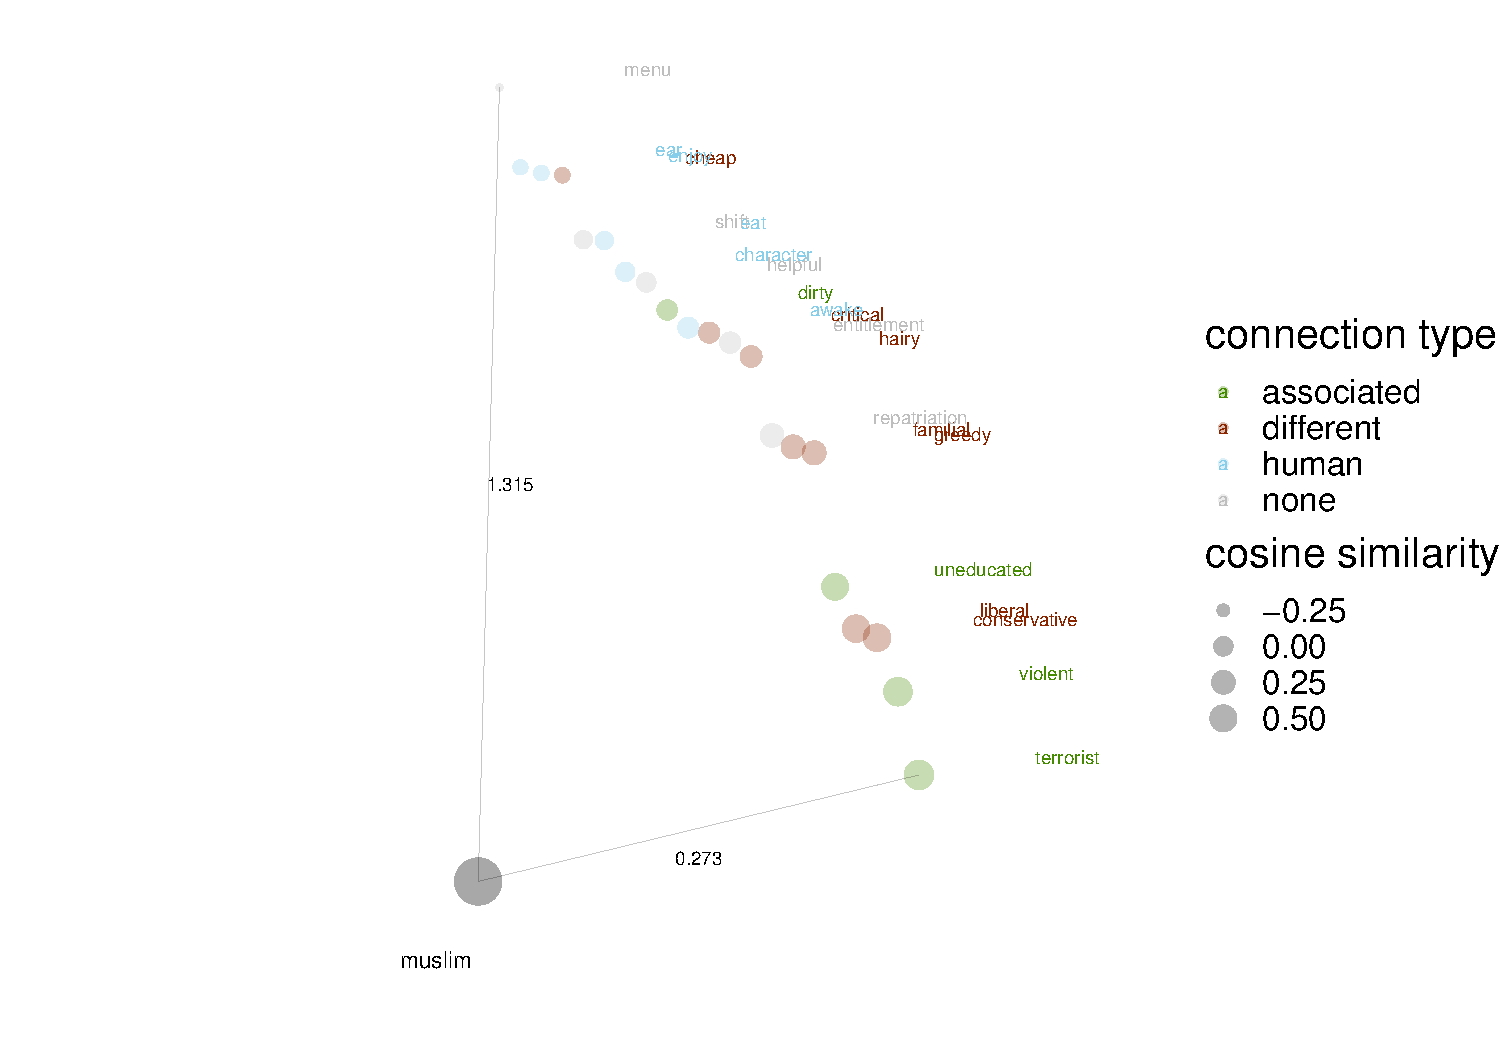
\includegraphics[width=0.8\linewidth]{presentationBoston_files/figure-beamer/unnamed-chunk-4-1} \end{center}
\end{block}
\end{frame}

\begin{frame}{Some methodological problems}
\protect\hypertarget{some-methodological-problems-5}{}
\begin{block}{Distances for ``priest''}
\protect\hypertarget{distances-for-priest}{}
\begin{center}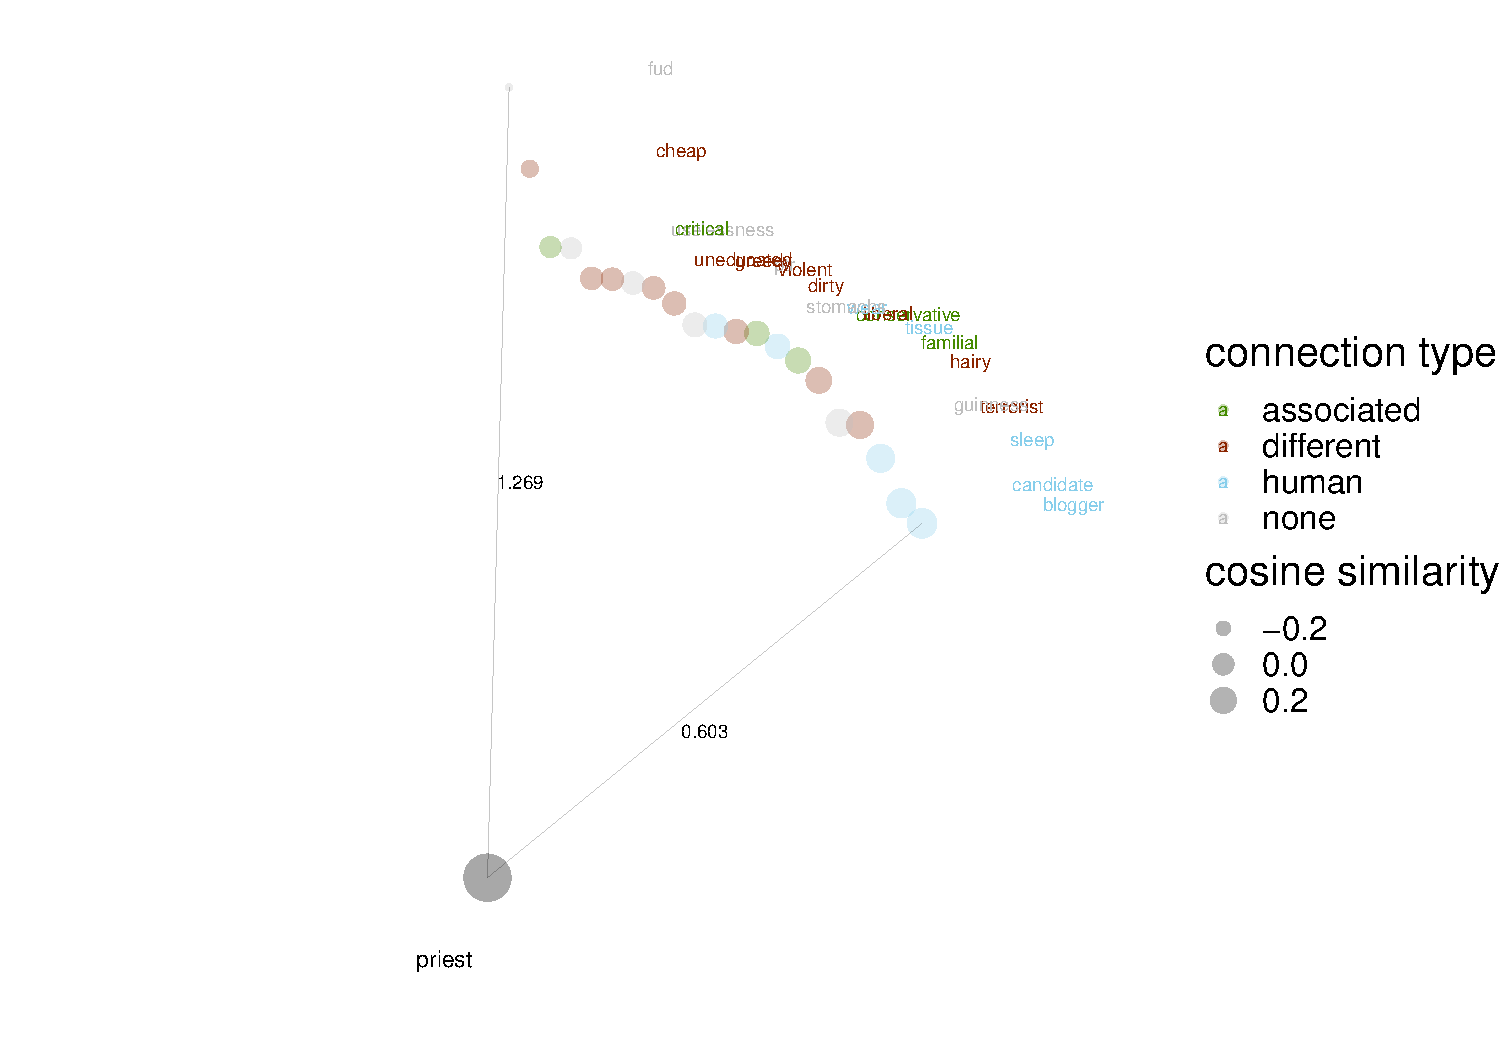
\includegraphics[width=0.8\linewidth]{presentationBoston_files/figure-beamer/unnamed-chunk-5-1} \end{center}
\end{block}
\end{frame}

\begin{frame}{Some methodological problems}
\protect\hypertarget{some-methodological-problems-6}{}
\begin{block}{No principled interpretation}
\protect\hypertarget{no-principled-interpretation}{}
\begin{longtable}[]{@{}lllll@{}}
\toprule
Category & Biased & Hard Debiased & Soft Debiased & Diff \\
\midrule
\endhead
Religion & 0.859 & 0.934 & 0.894 & 0.075 \\
Race & 0.892 & 0.925 & 0.985 & 0.033 \\
Gender & 0.623 & 0.700 & 0.747 & 0.077 \\
\bottomrule
\end{longtable}

\begin{itemize}
\item
  What values are sufficient for the presence of bias and what
  differences are sign of real improvement?
\item
  Low \(p\)-values are not high effect indicators!
\item
  We compare HPDIs.
\end{itemize}
\end{block}
\end{frame}

\begin{frame}{The problem with pre-averaging}
\protect\hypertarget{the-problem-with-pre-averaging}{}
\begin{block}{Key conceptual issues}
\protect\hypertarget{key-conceptual-issues}{}
\begin{itemize}
\tightlist
\item
  It throws away information about sample sizes
\item
  It ignores variation in the raw data, which leads to false confidence
\end{itemize}

\pause
\end{block}

\begin{block}{Our simulations}
\protect\hypertarget{our-simulations}{}
Suppose all similarities for two classes are randomly drawn from the
same distribution, \(\mathsf{Normal}(\mu = 0, \sigma = .08)\), you still
can get a really high WEAT!
\end{block}
\end{frame}

\begin{frame}{The problem with pre-averaging}
\protect\hypertarget{the-problem-with-pre-averaging-1}{}
\begin{block}{Simple case: two pws, four terms}
\protect\hypertarget{simple-case-two-pws-four-terms}{}
\vspace{1mm}
\footnotesize

\begin{center}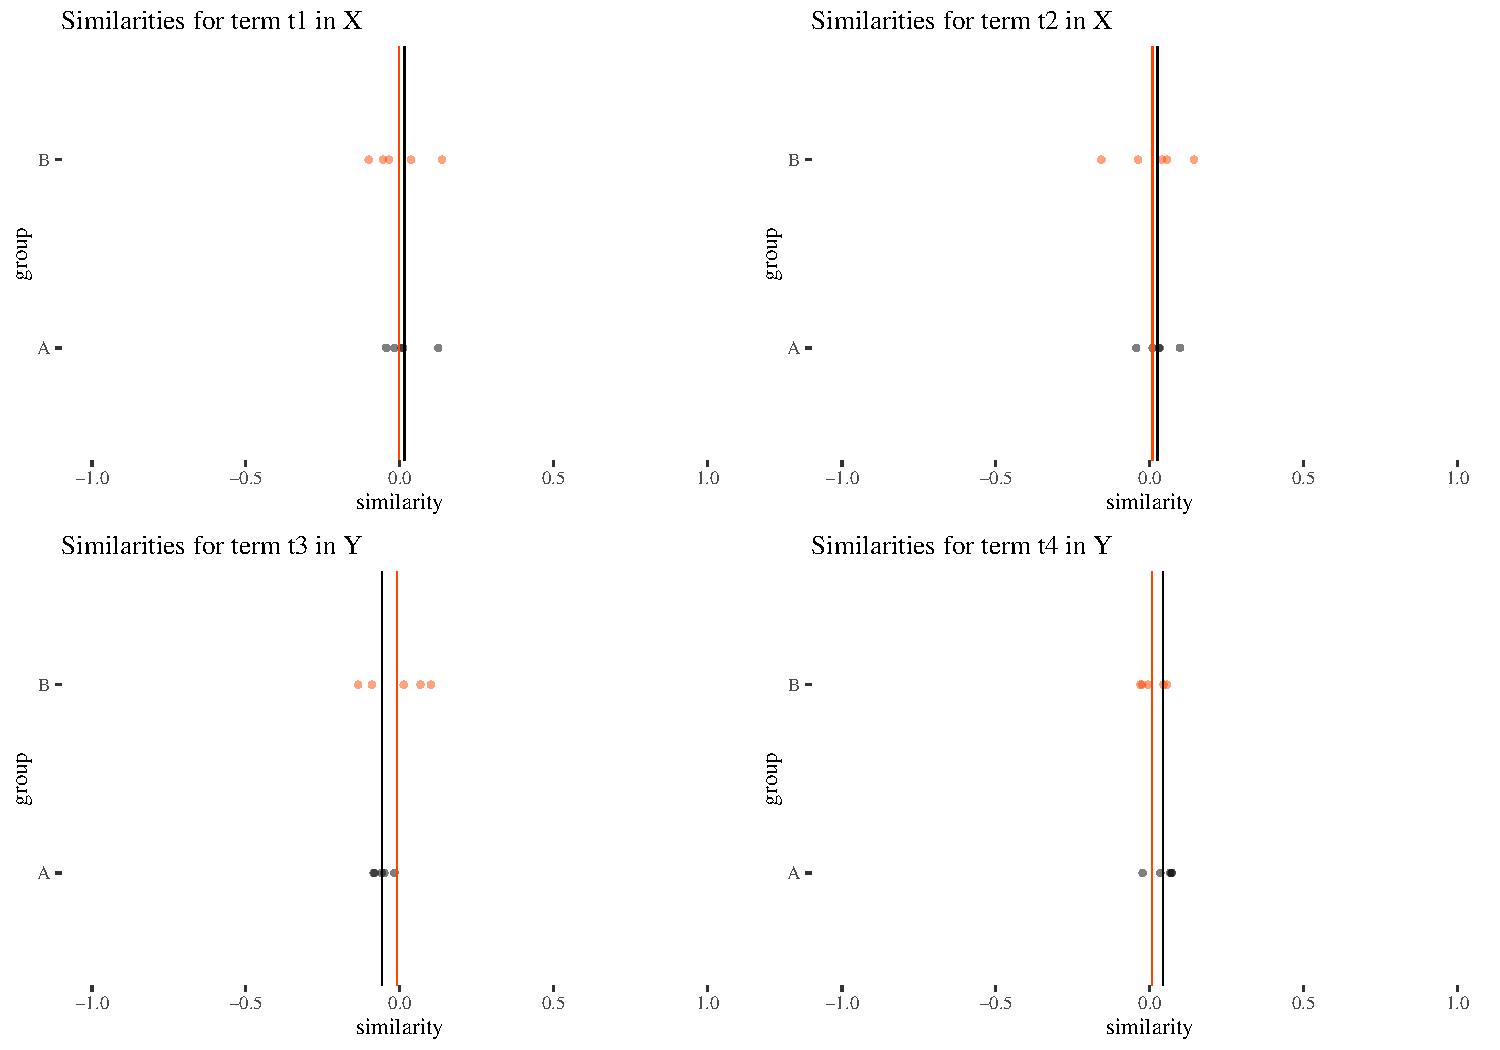
\includegraphics[width=0.7\linewidth]{presentationBoston_files/figure-beamer/unnamed-chunk-6-1} \end{center}
\normalsize

\vspace{1mm}
\footnotesize

\normalsize
\pause

\footnotesize

\vspace{-2mm}

\begin{itemize}
\tightlist
\item
  Raw sd in data is 0.072
\item
  The sd of means is 0.037
\item
  The WEAT score is 1.825\\
\item
  The largest effect size reported by
  \protect\hyperlink{ref-Caliskan2017semanticsBiases}{Caliskan, Bryson,
  \& Narayanan}
  (\protect\hyperlink{ref-Caliskan2017semanticsBiases}{2017}) is 1.81!
\end{itemize}
\end{block}
\end{frame}

\begin{frame}{The problem with pre-averaging on realistic set-up}
\protect\hypertarget{the-problem-with-pre-averaging-on-realistic-set-up}{}
\begin{block}{Simulation with realistic set-up (16 predicates)}
\protect\hypertarget{simulation-with-realistic-set-up-16-predicates}{}
\vspace{1mm}
\footnotesize

\begin{center}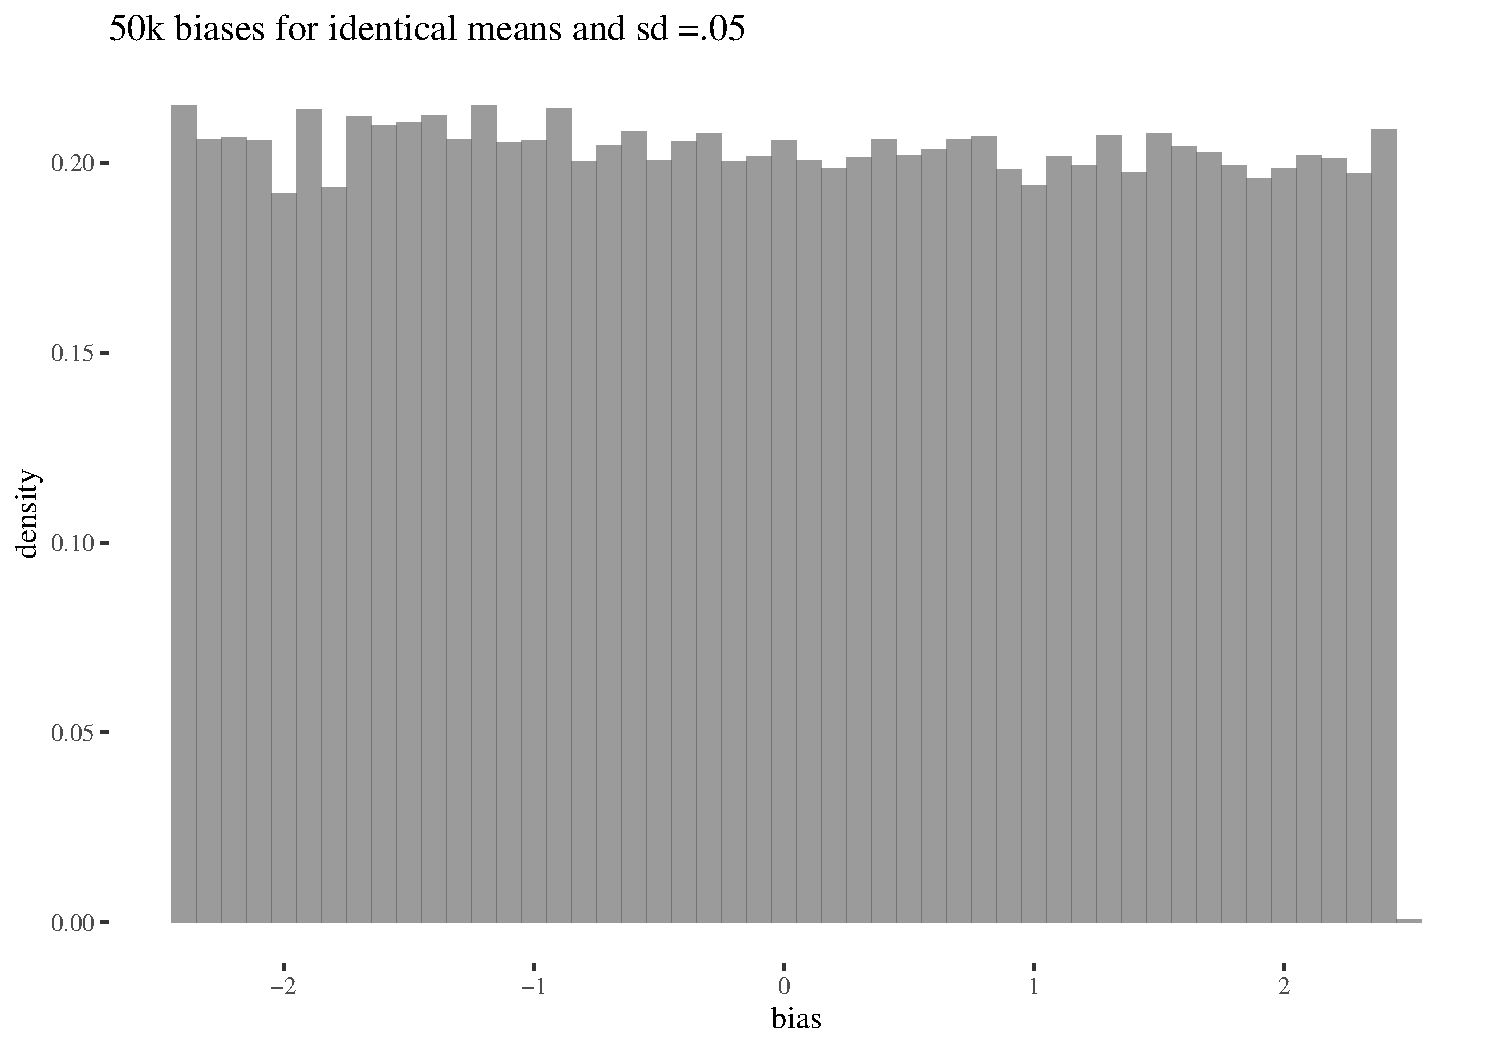
\includegraphics[width=0.7\linewidth]{presentationBoston_files/figure-beamer/unnamed-chunk-8-1} \end{center}

\footnotesize

\vspace{-2mm}

Raw sd: 0.082, sd of means: 0.031, WEAT: 2.337.
\end{block}
\end{frame}

\begin{frame}{The problem with pre-averaging on realistic set-up}
\protect\hypertarget{the-problem-with-pre-averaging-on-realistic-set-up-1}{}
\begin{block}{10k simulations (same parameters)}
\protect\hypertarget{k-simulations-same-parameters}{}
\vspace{1mm}
\footnotesize

\begin{center}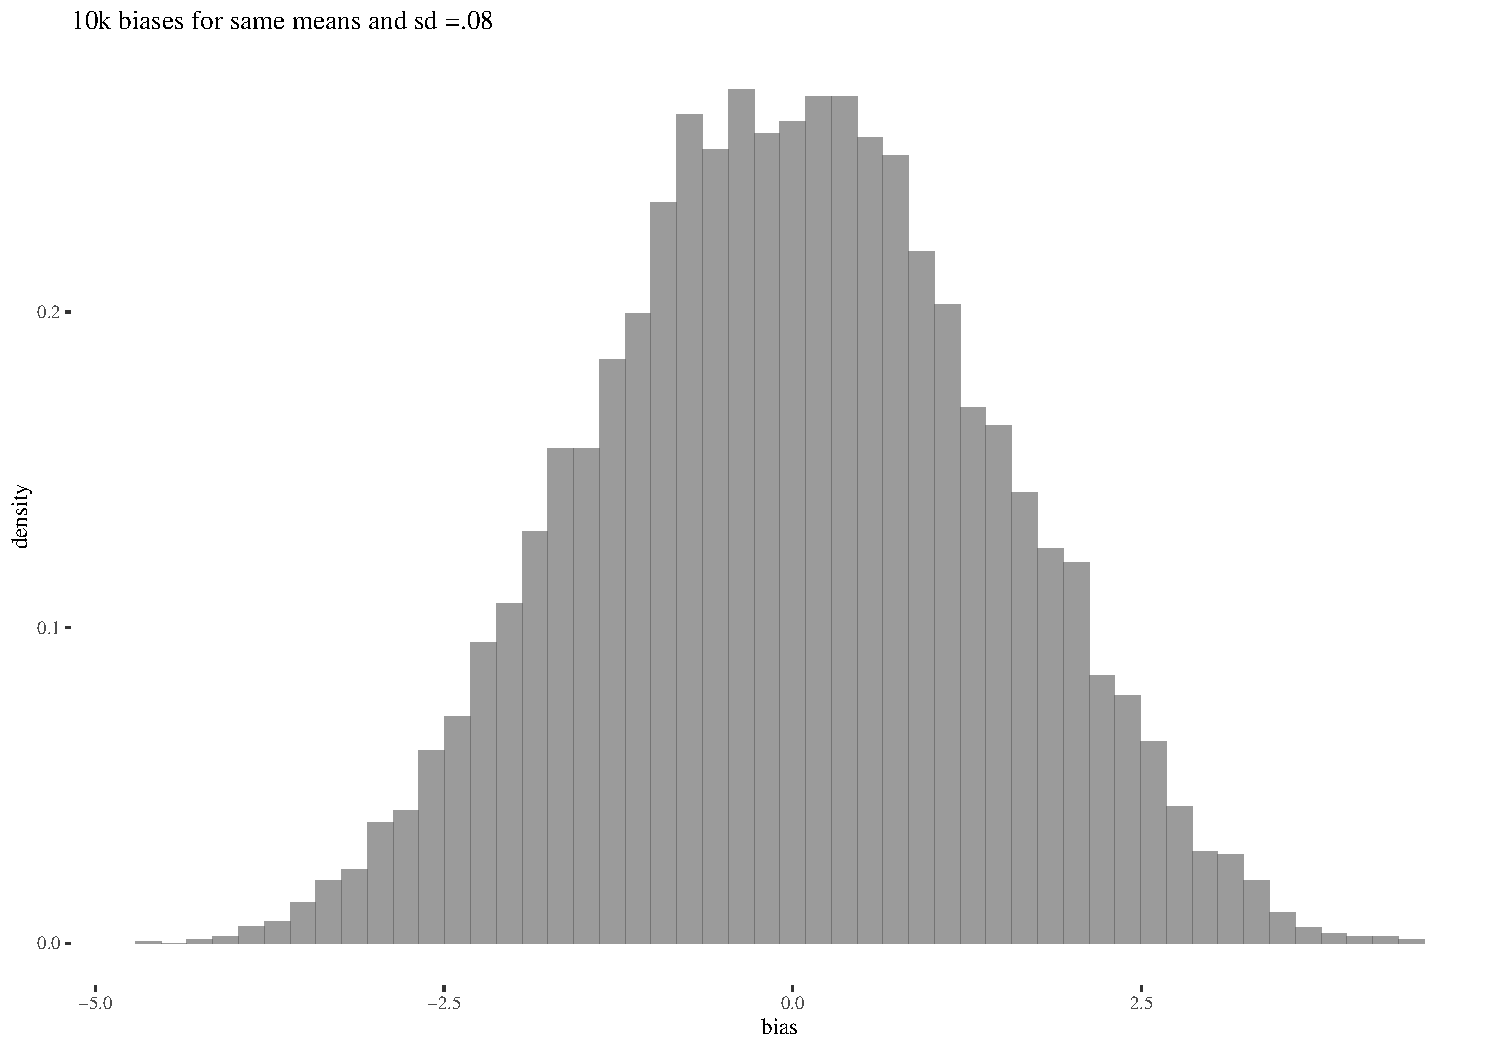
\includegraphics[width=0.8\linewidth]{presentationBoston_files/figure-beamer/unnamed-chunk-9-1} \end{center}
\vspace{1mm}
\footnotesize

\normalsize
\pause

\footnotesize

\vspace{-2mm}

\begin{itemize}
\tightlist
\item
  95\% of the scores are in range -2.763, 2.698
\item
  21.38\% of the absolute values are above 1.81
\end{itemize}
\end{block}
\end{frame}

\begin{frame}{The problem with pre-averaging on realistic set-up}
\protect\hypertarget{the-problem-with-pre-averaging-on-realistic-set-up-2}{}
\begin{block}{10k simulations with mean similarity 0.1}
\protect\hypertarget{k-simulations-with-mean-similarity-0.1}{}
\vspace{1mm}
\footnotesize

\begin{center}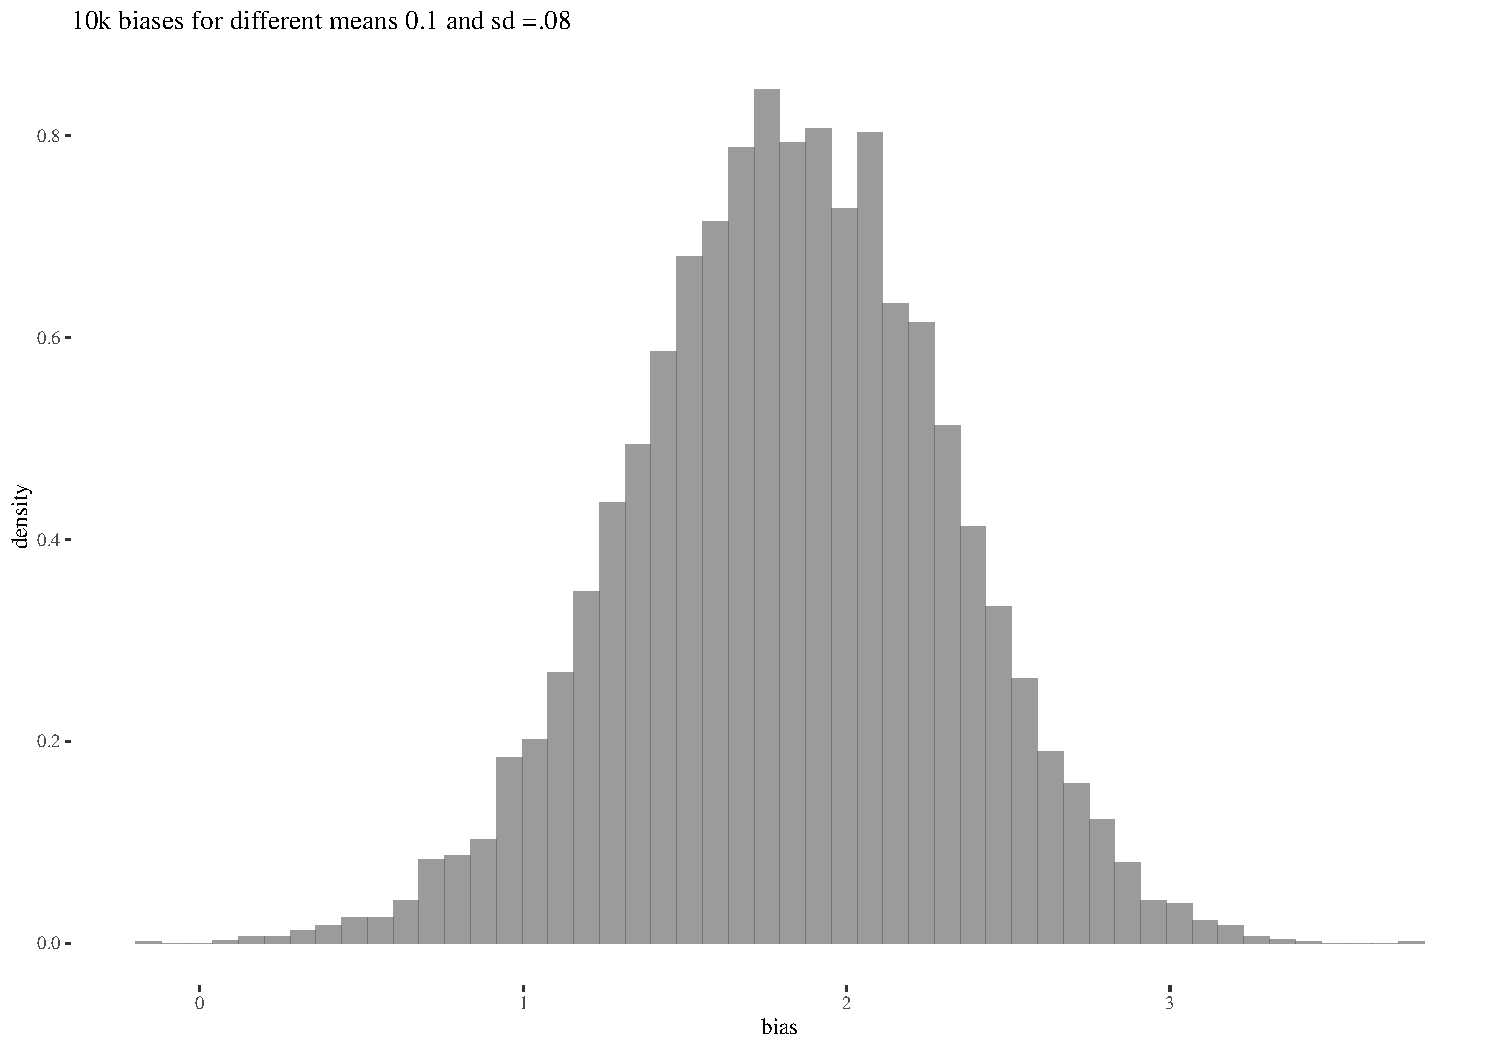
\includegraphics[width=0.8\linewidth]{presentationBoston_files/figure-beamer/unnamed-chunk-11-1} \end{center}
\vspace{1mm}
\footnotesize

\normalsize

\footnotesize

\vspace{-2mm}

\begin{itemize}
\tightlist
\item
  95\% of the scores are in range 0.851, 2.764
\item
  51.3\% of the absolute values are above 1.81
\end{itemize}
\end{block}
\end{frame}

\begin{frame}{The problem with pre-averaging on realistic set-up}
\protect\hypertarget{the-problem-with-pre-averaging-on-realistic-set-up-3}{}
\begin{block}{10k simulations with mean similarity 0.4}
\protect\hypertarget{k-simulations-with-mean-similarity-0.4}{}
\vspace{1mm}
\footnotesize

\begin{center}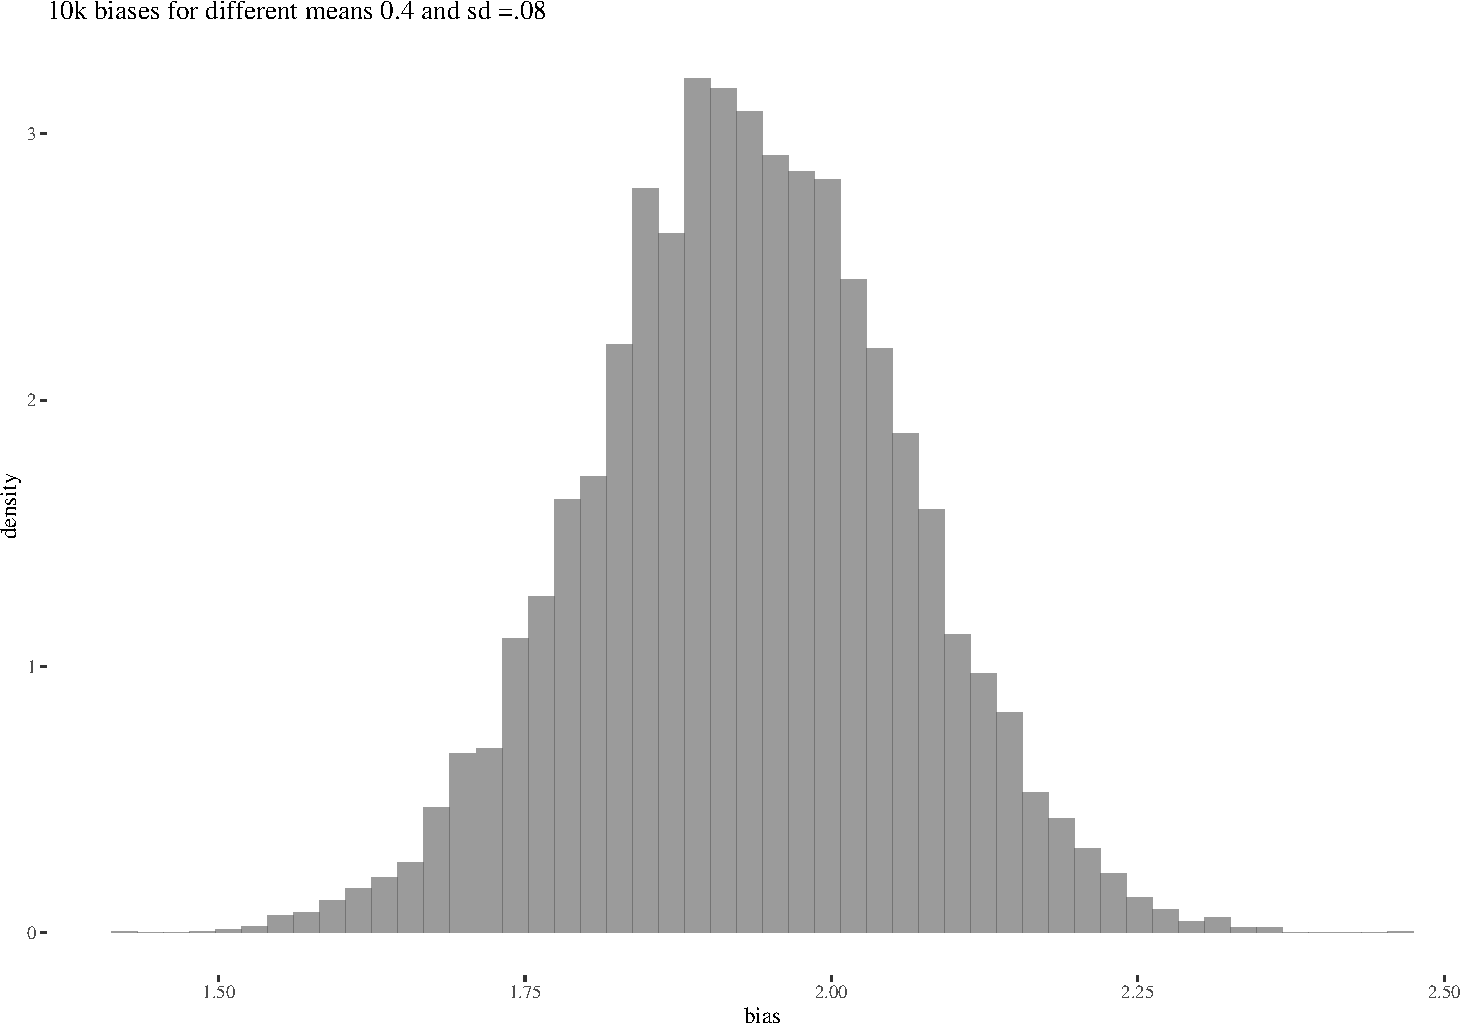
\includegraphics[width=0.8\linewidth]{presentationBoston_files/figure-beamer/unnamed-chunk-13-1} \end{center}
\vspace{1mm}
\footnotesize

\normalsize

\footnotesize

\vspace{-2mm}

\begin{itemize}
\tightlist
\item
  95\% of the scores are in range 1.679, 2.185
\item
  82.9\% of the absolute values are above 1.81
\end{itemize}
\end{block}
\end{frame}

\begin{frame}{Advantages of the Bayesian way}
\protect\hypertarget{advantages-of-the-bayesian-way}{}
\begin{itemize}
\tightlist
\item
  Direct impact of sample sizes
\item
  Straightforward interpretation in terms of posterior probabilities
\item
  Freedom to choose granularity level
\item
  More honest risk assessment and decision making
\end{itemize}
\end{frame}

\begin{frame}{Bayesian model}
\protect\hypertarget{bayesian-model}{}
\begin{block}{Choosing priors}
\protect\hypertarget{choosing-priors}{}
\begin{center}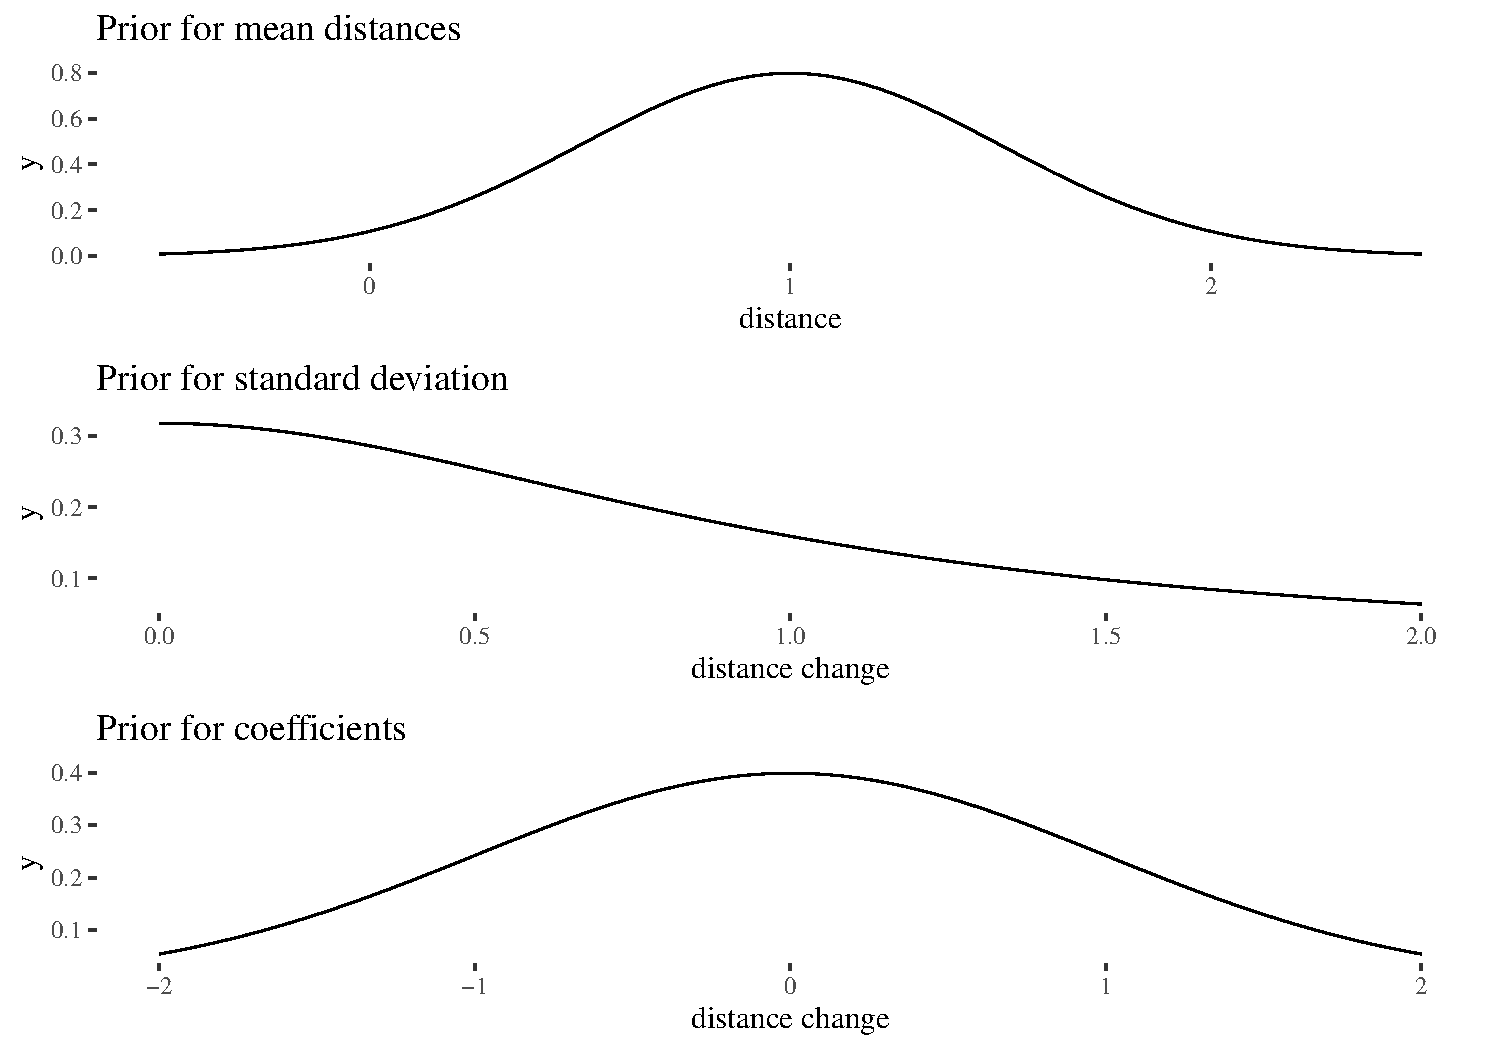
\includegraphics[width=1\linewidth]{presentationBoston_files/figure-beamer/priorsVis-1} \end{center}
\end{block}
\end{frame}

\begin{frame}[fragile]{Bayesian model architecture}
\protect\hypertarget{bayesian-model-architecture}{}
\vspace{1mm}
\footnotesize

\begin{Shaded}
\begin{Highlighting}[]
\FunctionTok{library}\NormalTok{(rethinking)}
\FunctionTok{options}\NormalTok{(}\AttributeTok{buildtools.check =} \ControlFlowTok{function}\NormalTok{(action) }\ConstantTok{TRUE}\NormalTok{ )}
\NormalTok{religionCoefs }\OtherTok{\textless{}{-}} \FunctionTok{ulam}\NormalTok{(}
  \FunctionTok{alist}\NormalTok{(}
\NormalTok{    cosineDistance }\SpecialCharTok{\textasciitilde{}} \FunctionTok{dnorm}\NormalTok{(mu,sigma),}
\NormalTok{    mu }\OtherTok{\textless{}{-}}\NormalTok{ m }\SpecialCharTok{+}\NormalTok{ co[con],}
\NormalTok{    m }\SpecialCharTok{\textasciitilde{}} \FunctionTok{dnorm}\NormalTok{(}\DecValTok{1}\NormalTok{,.}\DecValTok{5}\NormalTok{),}
\NormalTok{    co[con] }\SpecialCharTok{\textasciitilde{}} \FunctionTok{dnorm}\NormalTok{(}\DecValTok{0}\NormalTok{,.}\DecValTok{5}\NormalTok{),}
\NormalTok{    sigma }\SpecialCharTok{\textasciitilde{}} \FunctionTok{dcauchy}\NormalTok{(}\DecValTok{0}\NormalTok{,}\DecValTok{1}\NormalTok{)}
\NormalTok{  ),}
  \AttributeTok{data =}\NormalTok{ religion,}
  \AttributeTok{chains=}\DecValTok{2}\NormalTok{ , }\AttributeTok{iter=}\DecValTok{8000}\NormalTok{ , }\AttributeTok{warmup=}\DecValTok{1000}\NormalTok{, }
  \AttributeTok{log\_lik =} \ConstantTok{TRUE}
\NormalTok{)}
\end{Highlighting}
\end{Shaded}

\normalsize
\end{frame}

\begin{frame}{Dataset-level coefficients}
\protect\hypertarget{dataset-level-coefficients}{}
\begin{block}{Religion with 89\%-compatibility intervals (HPDI)}
\protect\hypertarget{religion-with-89-compatibility-intervals-hpdi}{}
\begin{center}
\begin{figure}[!htb]\centering
   \begin{minipage}{0.55\textwidth}
  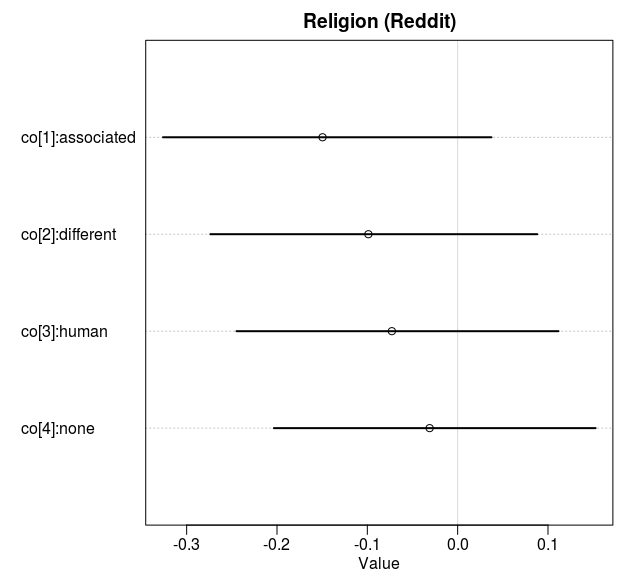
\includegraphics[width=6cm]{../../images/religionCoeffs.jpeg}
   \end{minipage} \begin{minipage}{0.4\textwidth}\footnotesize
   \begin{itemize}
   \item All HPDIs overlap with 0 
   \item Differences between classes are relatively small
   \item Coefficients for Race are similar
   \end{itemize}
   \end{minipage}
  \end{figure}
  
\end{center}
\end{block}
\end{frame}

\begin{frame}{Dataset-level coefficients}
\protect\hypertarget{dataset-level-coefficients-1}{}
\begin{block}{Gender with 89\%-compatibility intervals (HPDI)}
\protect\hypertarget{gender-with-89-compatibility-intervals-hpdi}{}
\begin{center}
\begin{figure}[!htb]\centering
  \begin{minipage}{0.55\textwidth}
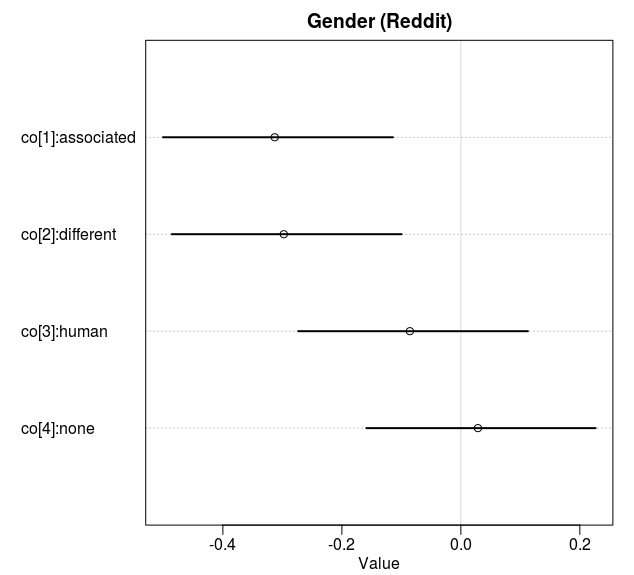
\includegraphics[width=6cm]{../../images/genderCoeffs.jpeg}
\end{minipage}
\begin{minipage}{0.4\textwidth}\footnotesize
   \begin{itemize}
   \item Associated and different are away from 0
   \item But they were supposed to be opposites and are very close to each other (co-occurrence?)
   \item Differences between classes are still relatively small
   \end{itemize}
   \end{minipage}
\end{figure}


\end{center}
\end{block}
\end{frame}

\begin{frame}[fragile]{Bayesian model architecture}
\protect\hypertarget{bayesian-model-architecture-1}{}
\vspace{1mm}
\footnotesize

\begin{Shaded}
\begin{Highlighting}[]
\FunctionTok{library}\NormalTok{(rethinking)}
\FunctionTok{options}\NormalTok{(}\AttributeTok{buildtools.check =} \ControlFlowTok{function}\NormalTok{(action) }\ConstantTok{TRUE}\NormalTok{ )}
\NormalTok{religionCoefs }\OtherTok{\textless{}{-}} \FunctionTok{ulam}\NormalTok{(}
  \FunctionTok{alist}\NormalTok{(}
\NormalTok{    cosineDistance }\SpecialCharTok{\textasciitilde{}} \FunctionTok{dnorm}\NormalTok{(mu,sigma),}
\NormalTok{    mu }\OtherTok{\textless{}{-}}\NormalTok{ m[pw] }\SpecialCharTok{+}\NormalTok{ co[con],}
\NormalTok{    m[pw] }\SpecialCharTok{\textasciitilde{}} \FunctionTok{dnorm}\NormalTok{(}\DecValTok{1}\NormalTok{,.}\DecValTok{5}\NormalTok{),}
\NormalTok{    co[con] }\SpecialCharTok{\textasciitilde{}} \FunctionTok{dnorm}\NormalTok{(}\DecValTok{0}\NormalTok{,.}\DecValTok{5}\NormalTok{),}
\NormalTok{    sigma }\SpecialCharTok{\textasciitilde{}} \FunctionTok{dcauchy}\NormalTok{(}\DecValTok{0}\NormalTok{,}\DecValTok{1}\NormalTok{)}
\NormalTok{  ),}
  \AttributeTok{data =}\NormalTok{ religion,}
  \AttributeTok{chains=}\DecValTok{2}\NormalTok{ , }\AttributeTok{iter=}\DecValTok{8000}\NormalTok{ , }\AttributeTok{warmup=}\DecValTok{1000}\NormalTok{, }
  \AttributeTok{log\_lik =} \ConstantTok{TRUE}
\NormalTok{)}
\end{Highlighting}
\end{Shaded}

\normalsize
\end{frame}

\begin{frame}{Word-level coefficients}
\protect\hypertarget{word-level-coefficients}{}
\begin{figure}[!htb]\centering
  \begin{minipage}{0.55\textwidth}
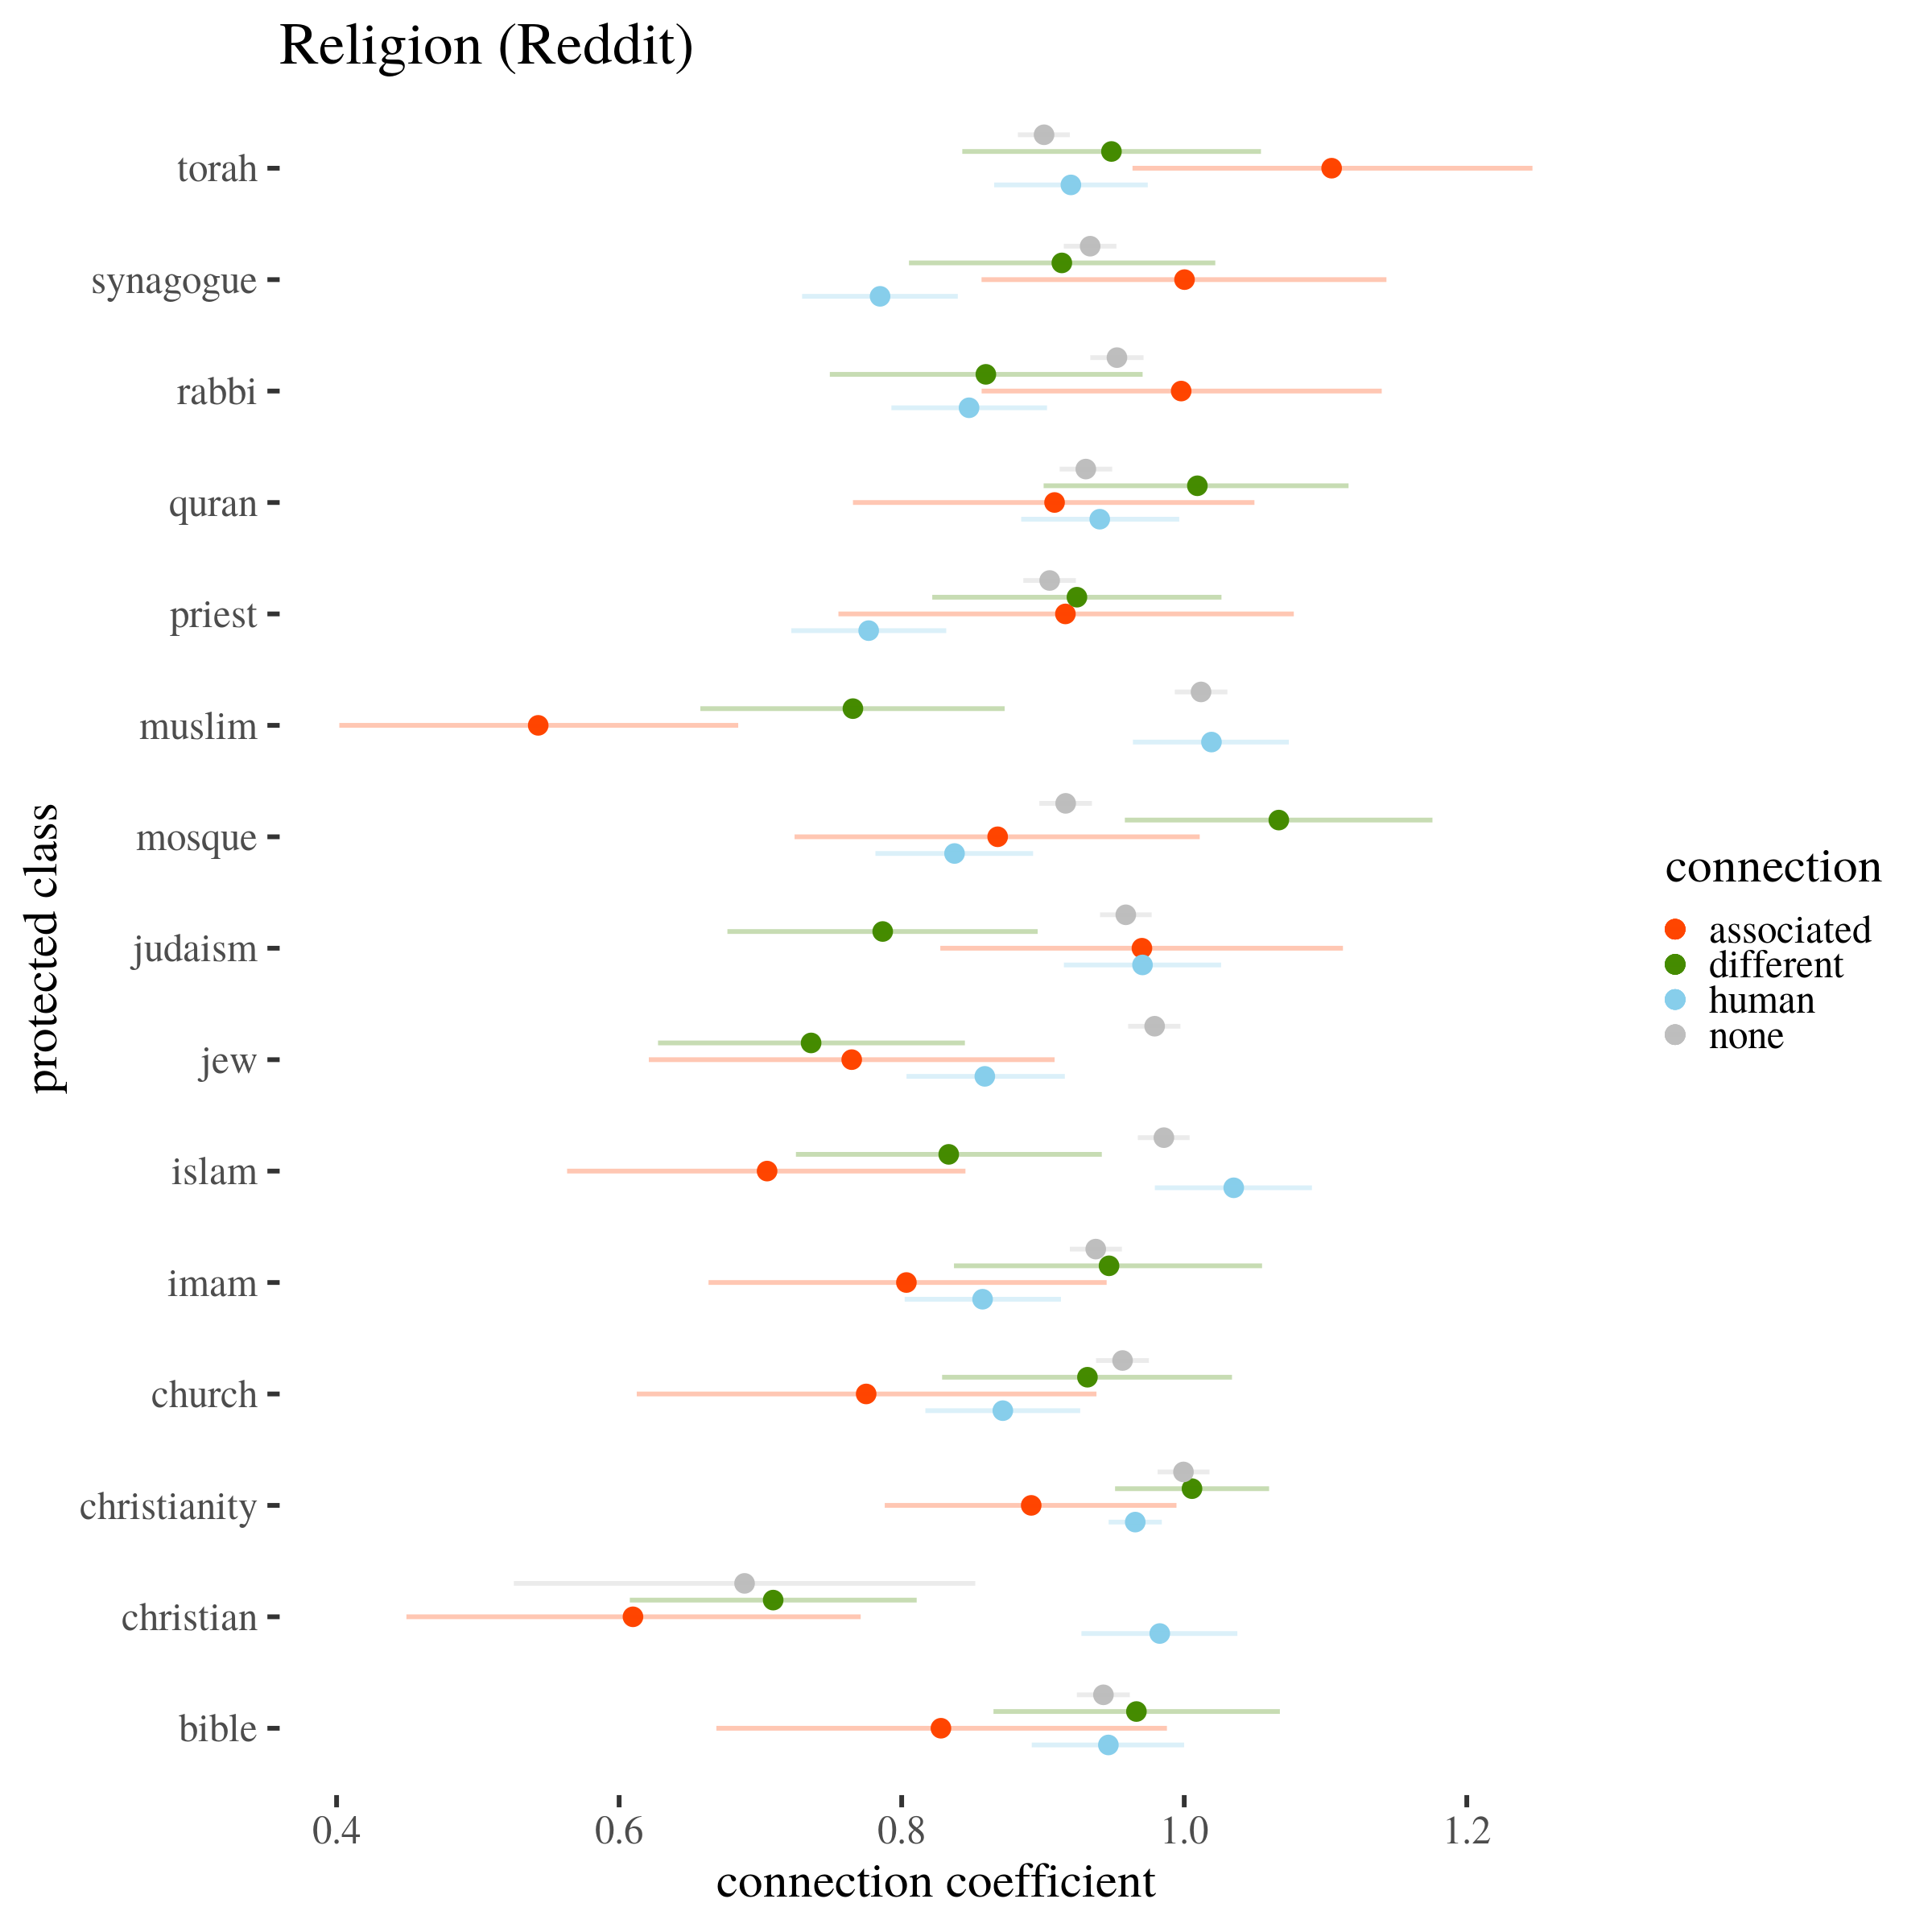
\includegraphics[width=7.5cm]{../../images/visReligionReddit.png}
\end{minipage}
\begin{minipage}{0.4\textwidth}\footnotesize

\vspace{-4cm}

   \begin{itemize}
   \item Most intervals overlap with control groups
   \item Often not too much difference between associated and different
   \end{itemize}
   \end{minipage}
\end{figure}
\end{frame}

\begin{frame}{Word-level coefficients}
\protect\hypertarget{word-level-coefficients-1}{}
\begin{figure}[!htb]\centering
  \begin{minipage}{0.55\textwidth}
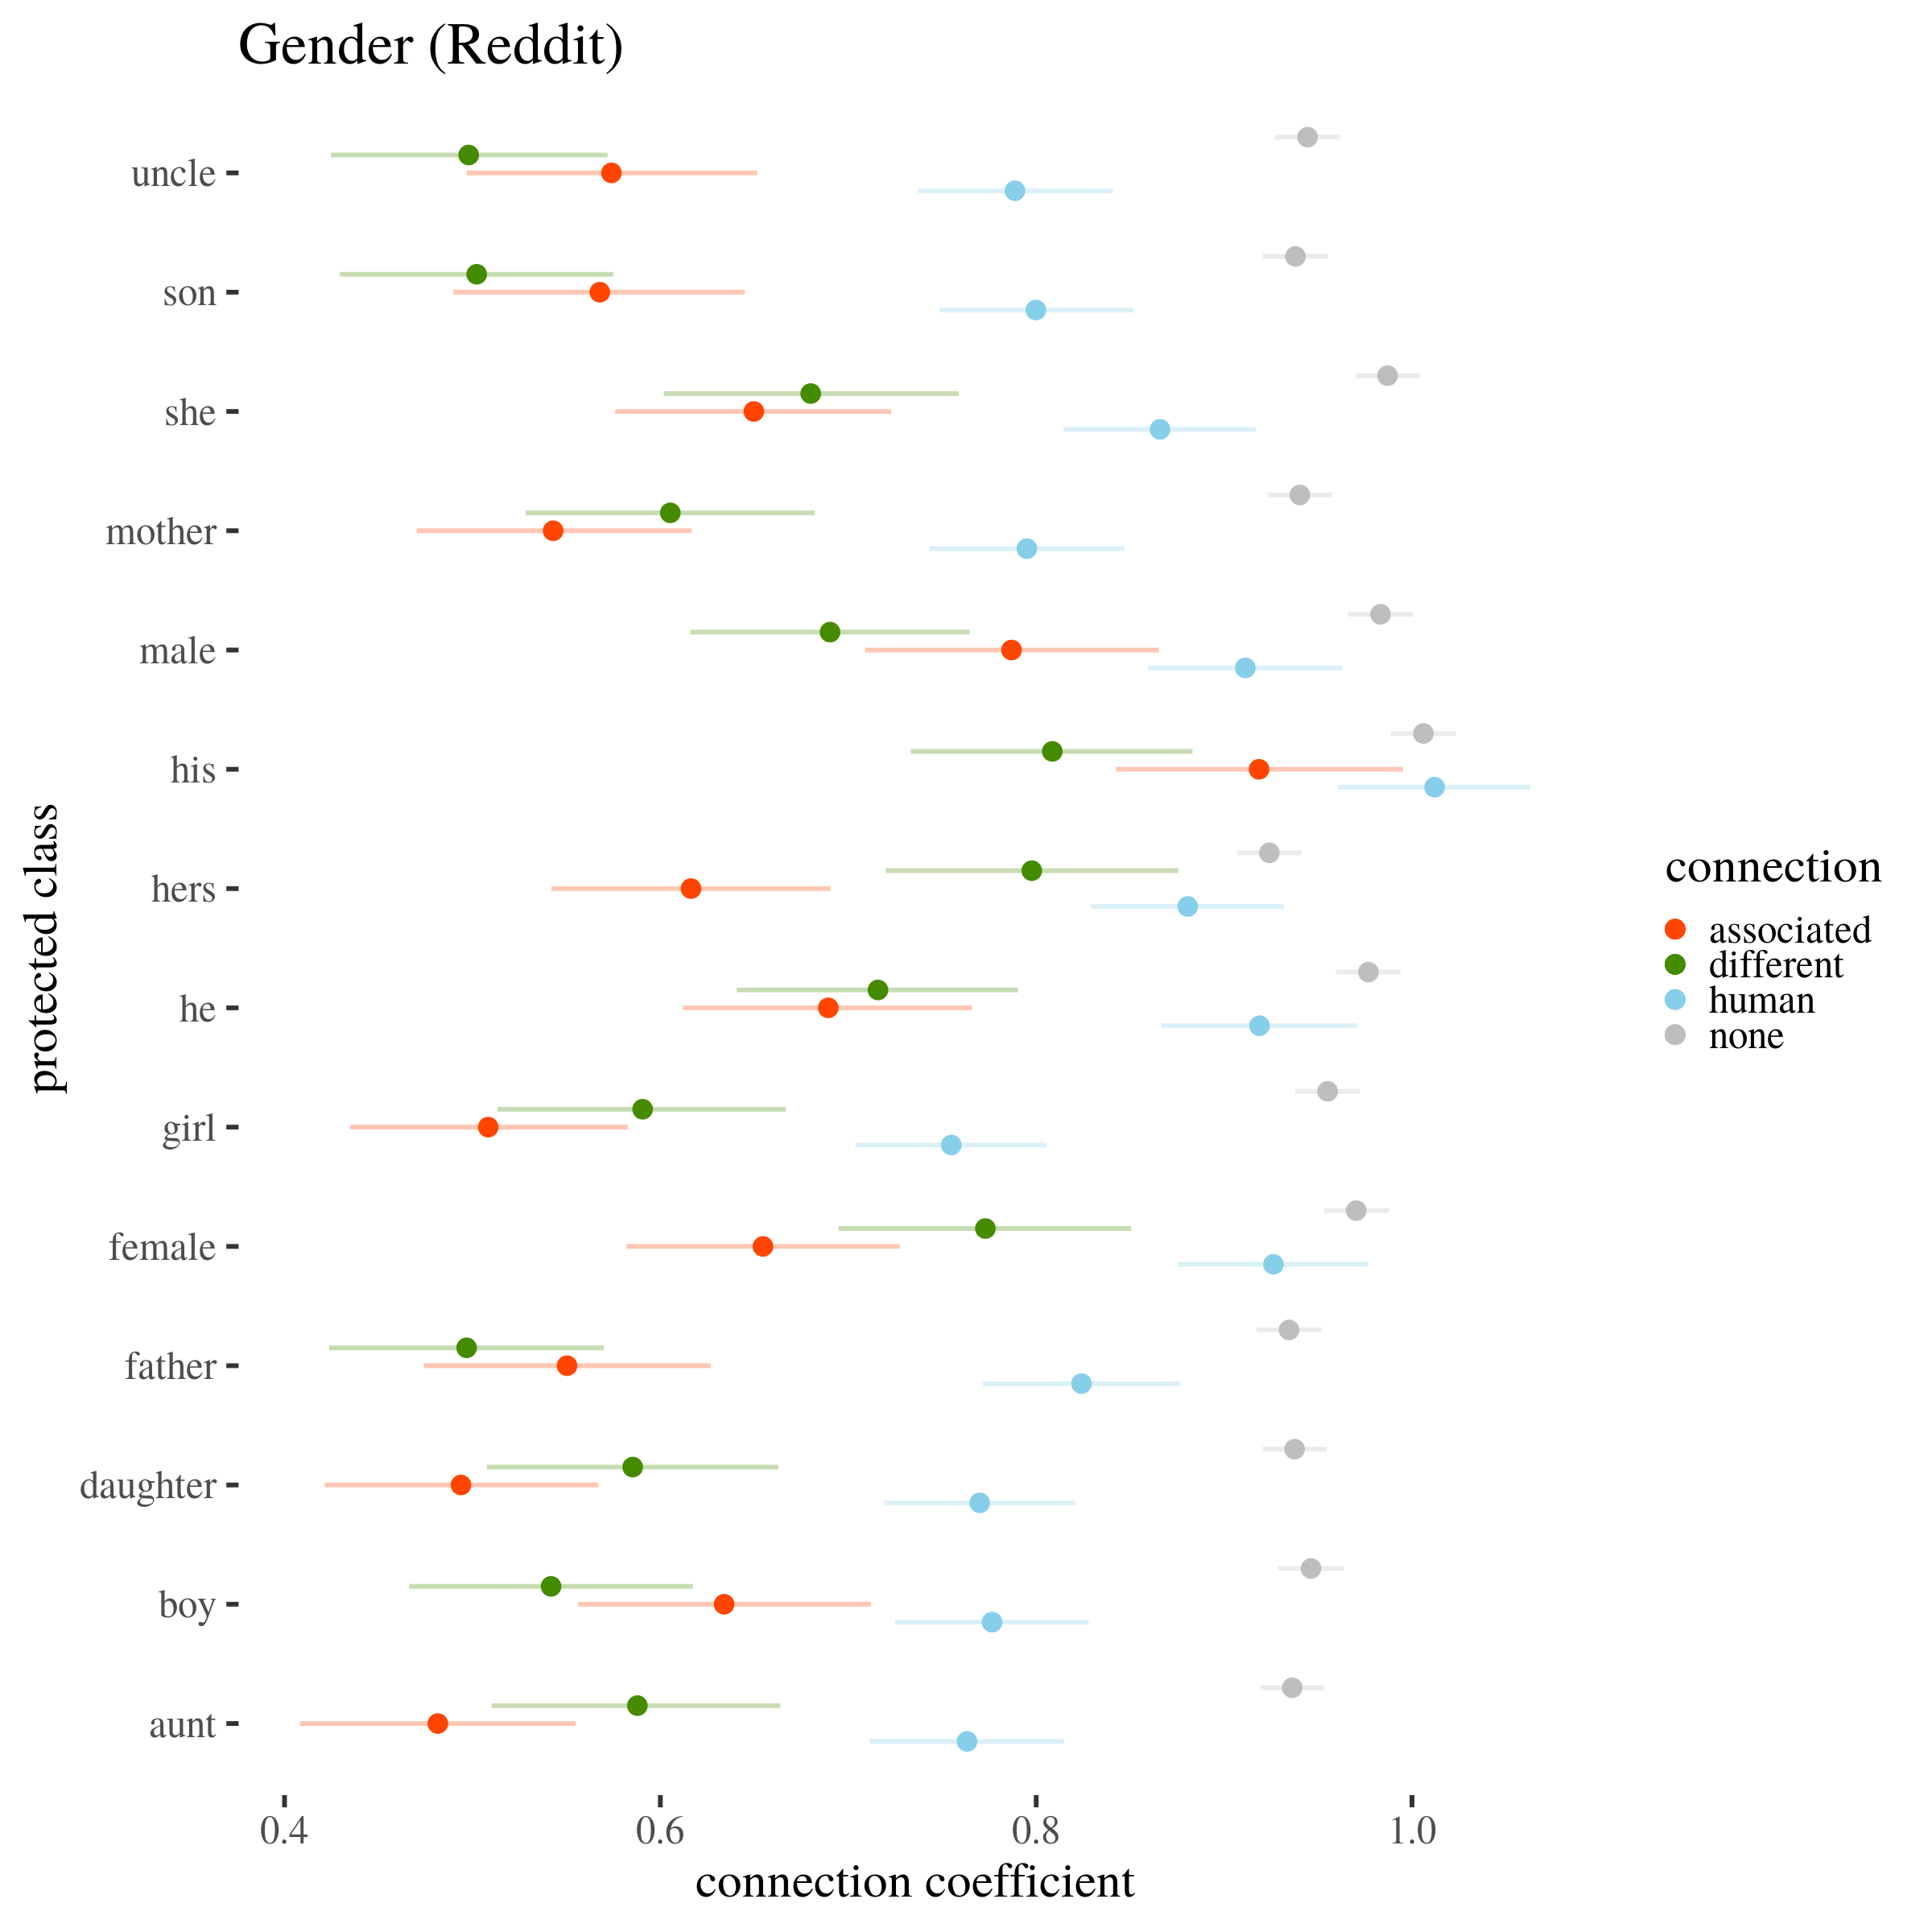
\includegraphics[width=7.5cm]{../../images/visGenderReddit.png}
\end{minipage}
\begin{minipage}{0.4\textwidth}\footnotesize

\vspace{-4cm}

   \begin{itemize}
   \item Male attributes: strong co-occurrence with female attributes
   \item Sometimes \textsf{different} is closer than \textsf{associated}
   \item Almost no overlap with control groups
   \end{itemize}
   \end{minipage}
\end{figure}
\end{frame}

\begin{frame}{Word-level coefficients}
\protect\hypertarget{word-level-coefficients-2}{}
\begin{figure}[!htb]\centering
  \begin{minipage}{0.55\textwidth}
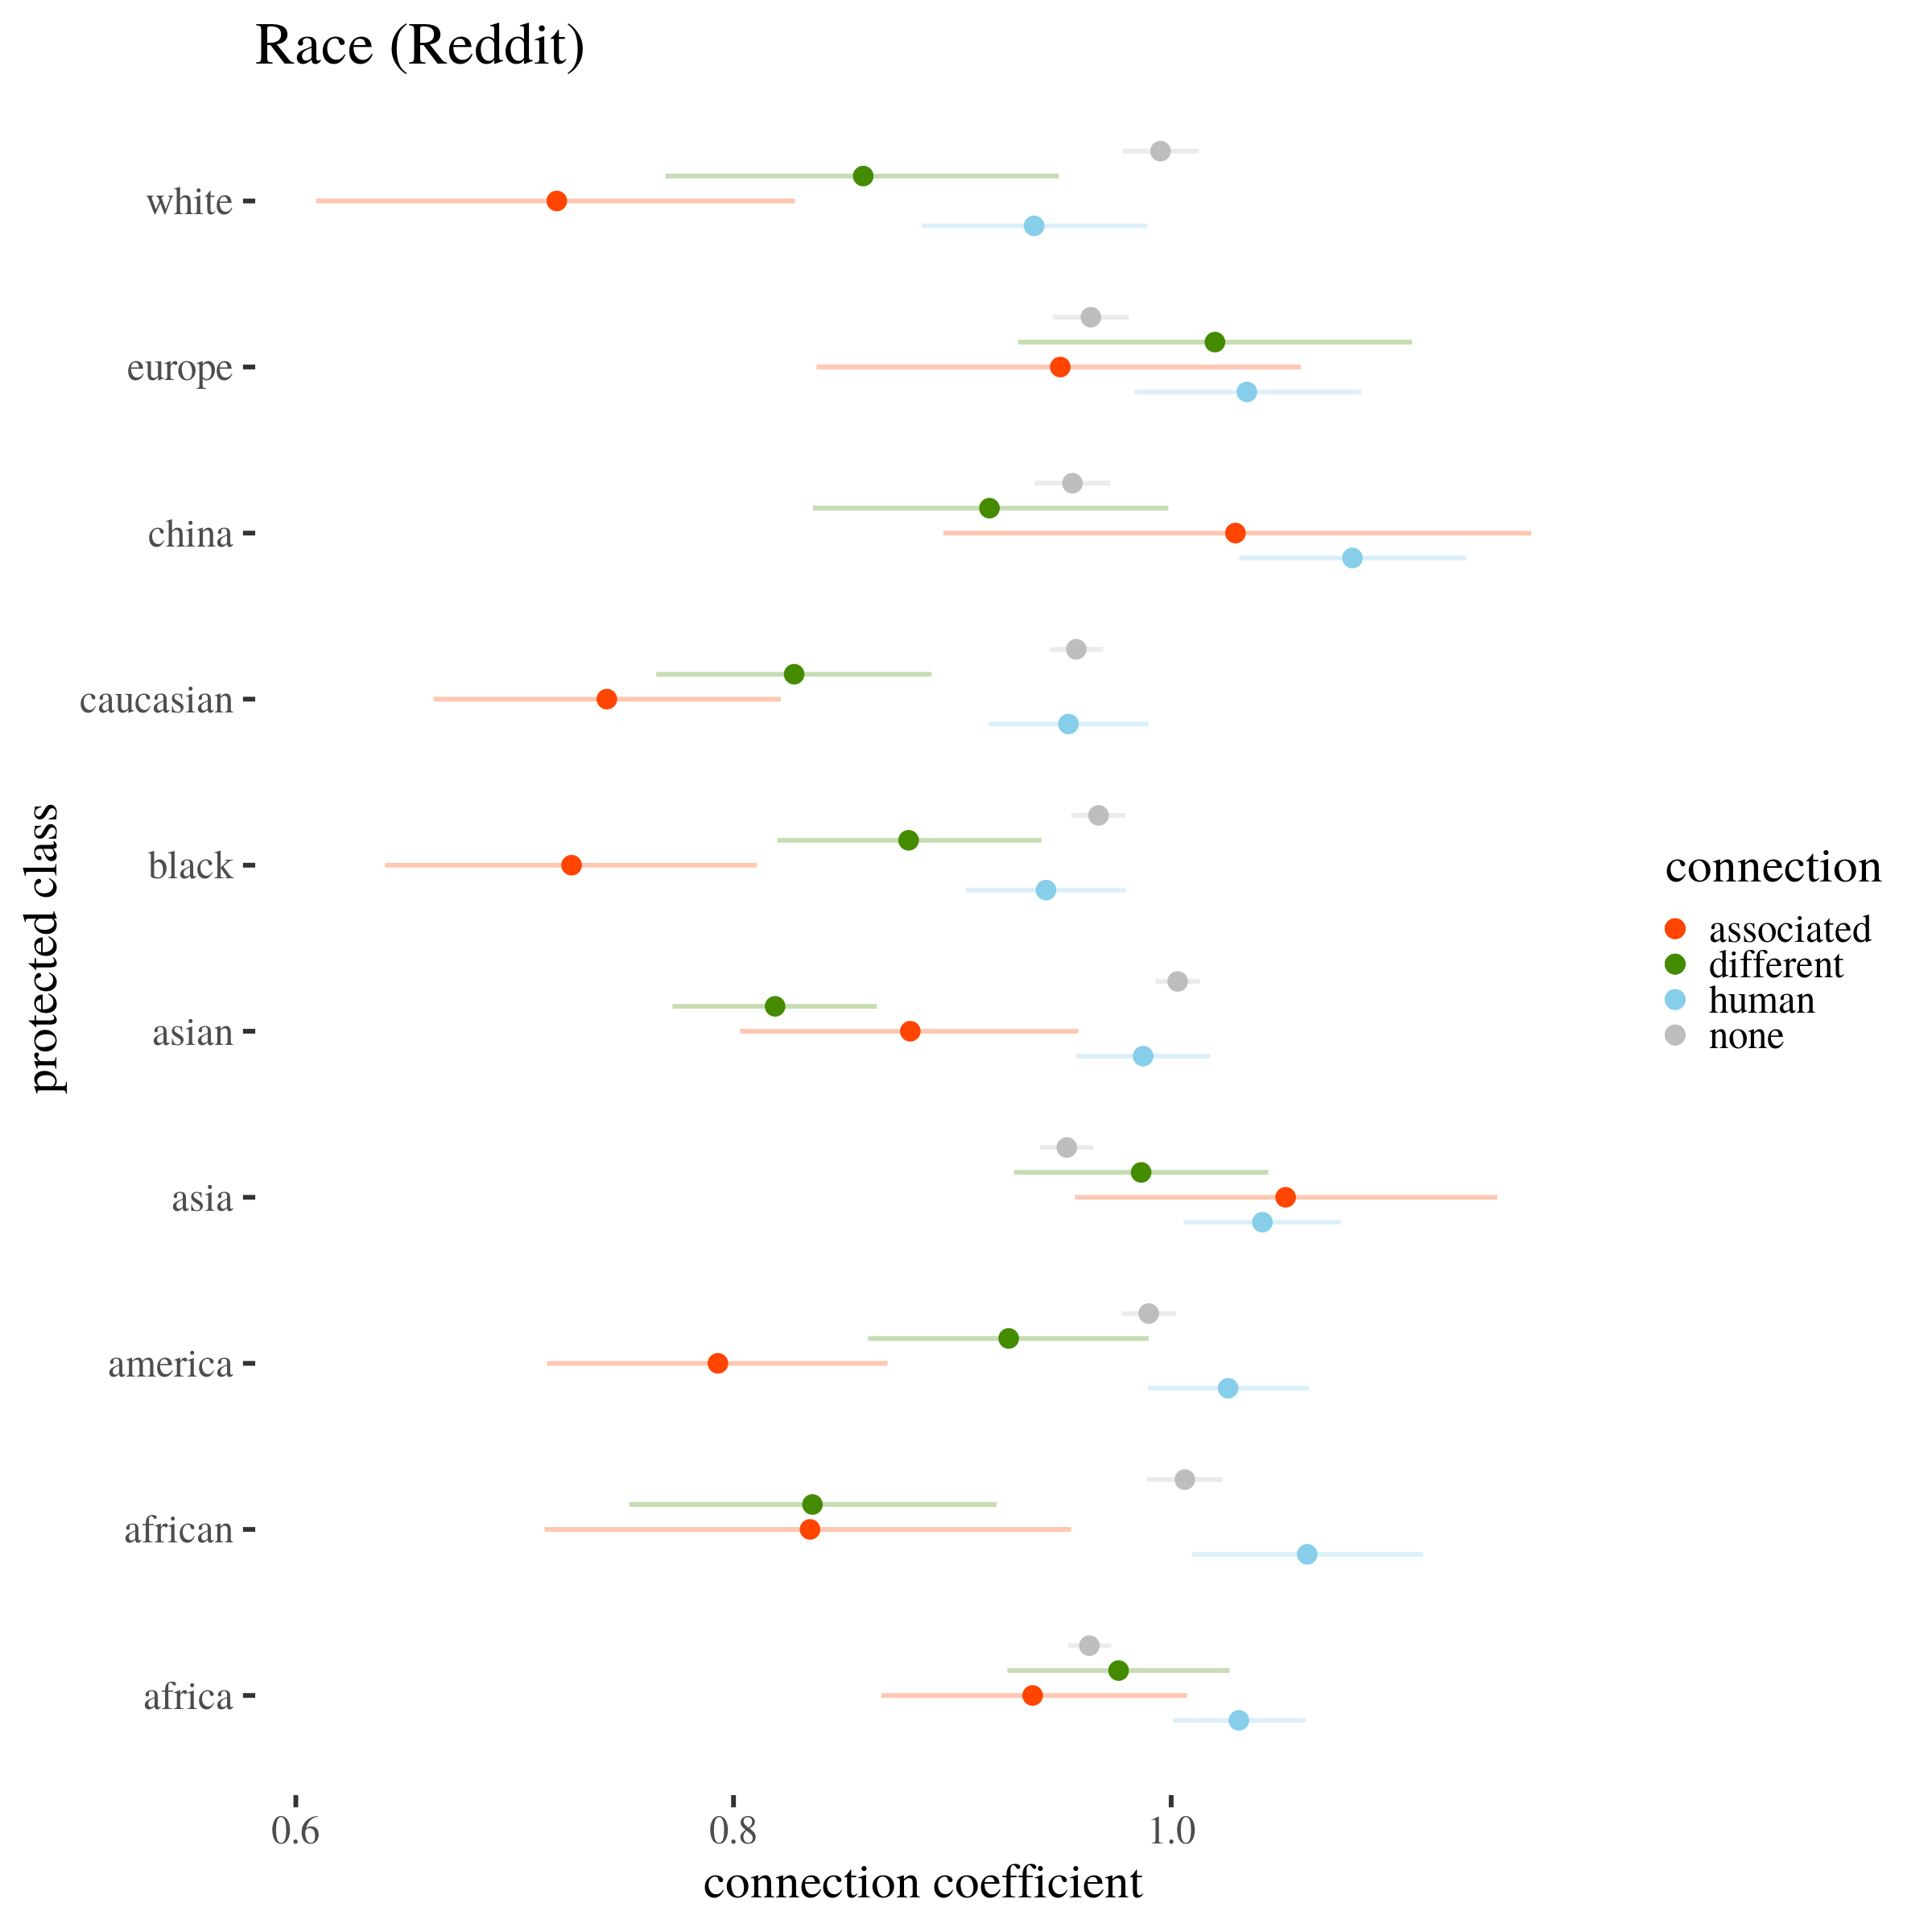
\includegraphics[width=7.5cm]{../../images/visRaceReddit.png}
\end{minipage}
\begin{minipage}{0.4\textwidth}\footnotesize

\vspace{-4cm}

   \begin{itemize}
   \item A lot of variation between races
   
   \item Often not much difference between associated and different
   \end{itemize}
   \end{minipage}
\end{figure}
\end{frame}

\begin{frame}{Thank you!}
\protect\hypertarget{thank-you}{}
\begin{block}{Summary}
\protect\hypertarget{summary}{}
\begin{itemize}
\tightlist
\item
  Bias in word embeddings
\item
  WEAT and MAC methods
\item
  Methodological problems
\item
  Limitations of pre-averaging in bias detection methods
\item
  Accounting for uncertainty with Bayesian approach
\end{itemize}
\end{block}

\begin{block}{Further work}
\protect\hypertarget{further-work}{}
\begin{itemize}
\tightlist
\item
  Including contrasts in Bayesian calculation
\item
  Performance cross-validation in comparison to other methods (regular
  linear regression, KNN, \dots)
\item
  Downstream tasks and connection with intrinsic evaluation
\item
  Testing data from the original Implicit Association Test (IAT)
\item
  Applying uncertainty to WEAT and better word lists
\item
  Looking at other similarity measures
\end{itemize}
\end{block}
\end{frame}

\begin{frame}{References}
\protect\hypertarget{references}{}
\tiny

\hypertarget{refs}{}
\begin{CSLReferences}{1}{0}
\leavevmode\hypertarget{ref-Caliskan2017semanticsBiases}{}%
Caliskan, A., Bryson, J. J., \& Narayanan, A. (2017). Semantics derived
automatically from language corpora contain human-like biases.
\emph{Science}, \emph{356}(6334), 183--186.
\url{https://doi.org/10.1126/science.aal4230}

\leavevmode\hypertarget{ref-Ethayarajh2020measuring}{}%
Ethayarajh, K. (2020). \emph{Is your classifier actually biased?
Measuring fairness under uncertainty with bernstein bounds}.

\leavevmode\hypertarget{ref-Ethayarajh2019understanding}{}%
Ethayarajh, K., Duvenaud, D., \& Hirst, G. (2019). Understanding
undesirable word embedding associations. \emph{Proceedings of the 57th
Annual Meeting of the Association for Computational Linguistics},
1696--1705.

\leavevmode\hypertarget{ref-Garg2018years}{}%
Garg, N., Schiebinger, L., Jurafsky, D., \& Zou, J. (2018). Word
embeddings quantify 100 years of gender and ethnic stereotypes.
\emph{Proceedings of the National Academy of Sciences}, \emph{115}(16),
E3635--E3644. \url{https://doi.org/10.1073/pnas.1720347115}

\leavevmode\hypertarget{ref-Gonen2019lipstick}{}%
Gonen, H., \& Goldberg, Y. (2019). Lipstick on a pig: {D}ebiasing
methods cover up systematic gender biases in word embeddings but do not
remove them. \emph{Proceedings of the 2019 Conference of the North
{A}merican Chapter of the Association for Computational Linguistics:
Human Language Technologies, Volume 1 (Long and Short Papers)},
609--614. Minneapolis, Minnesota: Association for Computational
Linguistics. \url{https://doi.org/10.18653/v1/N19-1061}

\leavevmode\hypertarget{ref-Lauscher2019multidimensional}{}%
Lauscher, A., \& Glavas, G. (2019). Are we consistently biased?
Multidimensional analysis of biases in distributional word vectors.
\emph{CoRR}, \emph{abs/1904.11783}. Retrieved from
\url{http://arxiv.org/abs/1904.11783}

\leavevmode\hypertarget{ref-Manzini2019blackToCriminal}{}%
Manzini, T., Lim, Y. C., Tsvetkov, Y., \& Black, A. W. (2019).
\emph{Black is to criminal as caucasian is to police: Detecting and
removing multiclass bias in word embeddings}. Retrieved from
\url{http://arxiv.org/abs/1904.04047}

\leavevmode\hypertarget{ref-Nissim2020fair}{}%
Nissim, M., Noord, R. van, \& Goot, R. van der. (2020). Fair is better
than sensational: Man is to doctor as woman is to doctor.
\emph{Computational Linguistics}, \emph{46}(2), 487--497.
\url{https://doi.org/10.1162/coli_a_00379}

\leavevmode\hypertarget{ref-zhang2020robustness}{}%
Zhang, H., Sneyd, A., \& Stevenson, M. (2020). \emph{Robustness and
reliability of gender bias assessment in word embeddings: The role of
base pairs}. Retrieved from \url{http://arxiv.org/abs/2010.02847}

\end{CSLReferences}
\end{frame}

\end{document}
